\documentclass[11pt,a4paper]{article}

\usepackage[margin=2.6cm]{geometry}
\usepackage{amsmath,amssymb,amsthm}
\usepackage{booktabs}
\usepackage{microtype}
\usepackage[hidelinks]{hyperref}
\usepackage{enumitem}
\usepackage{graphicx}
\usepackage{float}
\usepackage[font=small]{caption}
\usepackage{algorithm}
\usepackage{algpseudocode}
\graphicspath{{figs/}}

% The figures are wide screenshots and plots; let more than one share a page
% rather than each claiming its own.
\renewcommand{\topfraction}{0.92}
\renewcommand{\bottomfraction}{0.85}
\renewcommand{\textfraction}{0.06}
\renewcommand{\floatpagefraction}{0.72}

\newtheorem{proposition}{Proposition}
\newtheorem{remark}{Remark}
\newtheorem{definition}{Definition}

\newcommand{\R}{\mathbb{R}}
\newcommand{\Ec}{\eta_{\mathrm c}}
\newcommand{\Ed}{\eta_{\mathrm d}}
\newcommand{\dt}{\Delta t}

\title{Distributed Optimisation for Home Energy Management\\
\large Theory notes for \texttt{hems-policy}}
\author{}
\date{}

\begin{document}
\maketitle

\begin{abstract}
\noindent
These notes set out the optimisation problem solved by \texttt{hems-policy}, the
decomposition used to solve it, and the dual quantities the decomposition
produces as a by-product. Two coordinators are described: Dantzig--Wolfe, the
default, which collects plans from the devices, mixes them in a small linear
programme and certifies how far the result can be from the best plan; and
ADMM, which needs no linear programme and moves the devices toward agreement
through one shared price. Both feed the same Home Assistant and evcc
integrations. The emphasis is on the by-products: a dynamic
programming formulation yields a \emph{value function}, and its derivative in
the storage state is a price that can be published and consumed by devices the
optimiser never modelled. We state what is guaranteed, what is approximate, and
where the approximations were measured. Section~\ref{sec:limits} lists the
properties that do \emph{not} hold.
\end{abstract}

\paragraph{How to read these notes.} Section~\ref{sec:problem} states the
problem: a house with a meter, some devices, and a bill with different prices
for buying and selling. Section~\ref{sec:decomposition} splits it by device and
explains why the pieces need a coordinator; Section~\ref{sec:dw} coordinates
them with Dantzig--Wolfe, the default, and Section~\ref{sec:admm} with ADMM.
Section~\ref{sec:duals} explains the prices a plan comes with, and
Sections~\ref{sec:interplay} and~\ref{sec:integrations} how a plan reaches a real
house. Section~\ref{sec:compare} compares the two coordinators on measured
cases; Section~\ref{sec:limits} lists what is and is not guaranteed. Proofs,
full formulations and the supporting studies are in the appendices. Every
number quoted can be reproduced with a script in \texttt{bench/}.

Figure~\ref{fig:flows} shows the two coordinators side by side before any
detail. Both split the house by device and loop; they differ in what goes
round the loop, and in what the loop can say about its answer.


\tableofcontents
\clearpage

\begin{figure}[t]
\centering
\begin{minipage}[t]{0.48\textwidth}\centering
  \textbf{Dantzig--Wolfe} (Section~\ref{sec:dw})\\[4pt]
  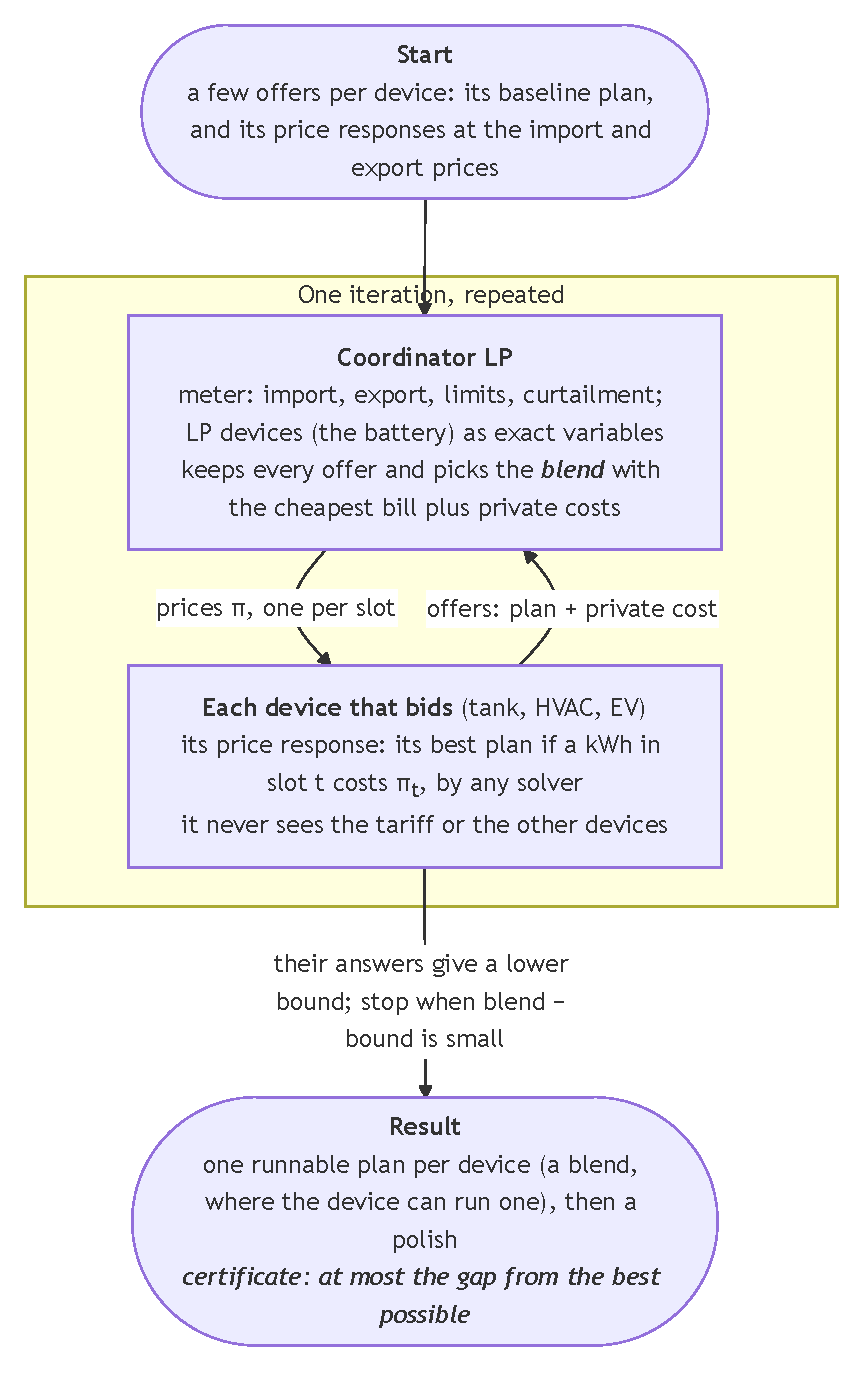
\includegraphics[width=\linewidth]{flow_dw.pdf}
\end{minipage}\hfill
\begin{minipage}[t]{0.48\textwidth}\centering
  \textbf{ADMM} (Section~\ref{sec:admm})\\[4pt]
  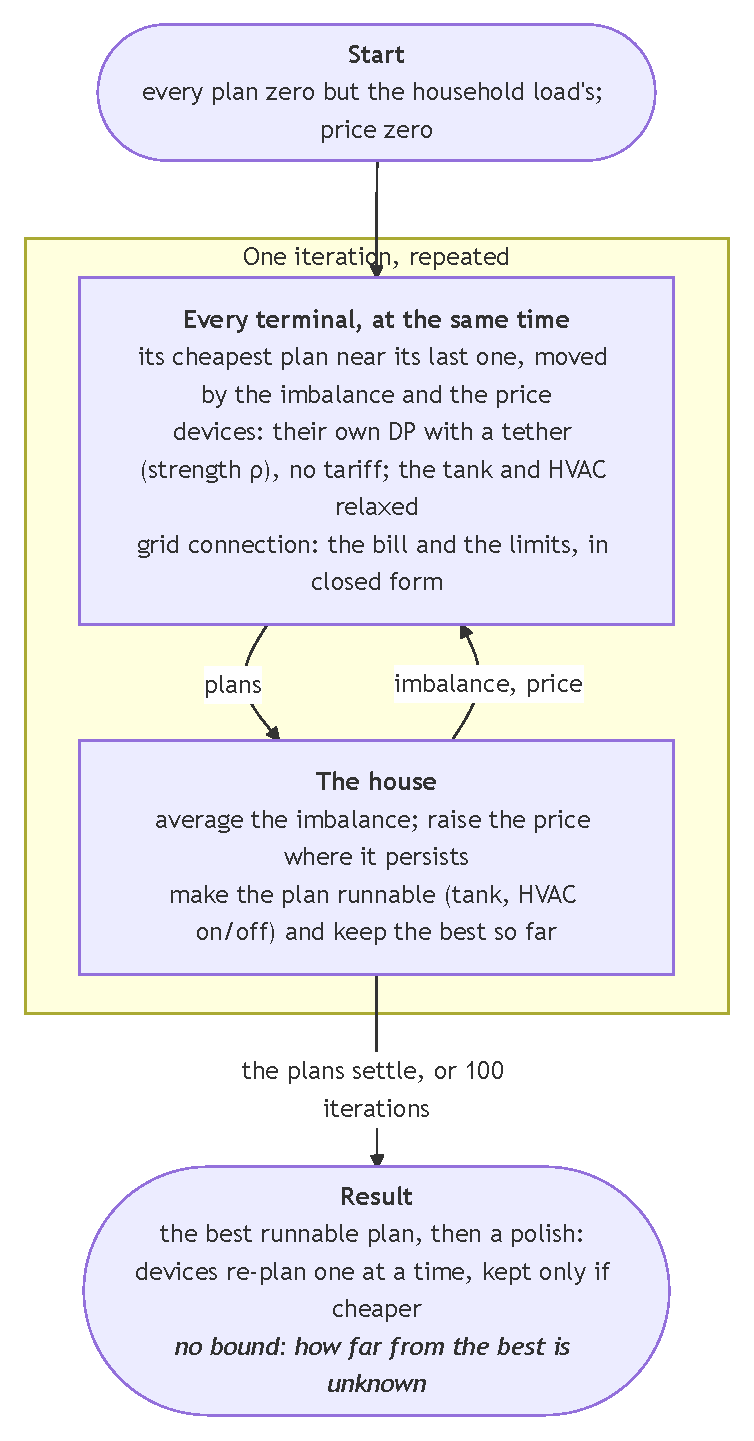
\includegraphics[width=\linewidth]{flow_admm.pdf}
\end{minipage}
\caption{What goes round each loop. \emph{Dantzig--Wolfe}: the coordinator's
LP, which holds the meter and the batteries exactly, posts one price per slot;
each remaining device answers with its best plan at that price, and the LP
blends the answers; the answers also give a lower bound, so the loop stops
with a certified gap. \emph{ADMM}: every device takes its cheapest plan near
its last one, moved by the house's imbalance and by a shared price that rises
where the imbalance persists, and the grid connection carries the bill; it
stops when the plans settle or the budget runs out, keeping the best runnable
plan, with no measure of how good it is. Sources:
\texttt{docs/figs/flow\_*.mmd} (Mermaid).}
\label{fig:flows}
\end{figure}

\section{The problem}
\label{sec:problem}

\subsection{Setting}

Time is discretised into $n$ slots of length $\dt$ hours, indexed
$t = 0,\dots,n-1$. Powers are in kW, energies in kWh, prices in currency per
kWh, temperatures in degrees Celsius; a slot spent at power $p$ therefore moves
$p\,\dt$ kWh. Exogenous data over the horizon:

\begin{center}
\begin{tabular}{lll}
\toprule
symbol & meaning & units \\
\midrule
$c^{\mathrm{imp}}_t$ & import tariff & currency/kWh \\
$c^{\mathrm{exp}}_t$ & export remuneration & currency/kWh \\
$\ell_t$ & inflexible household load & kW \\
$g_t$ & photovoltaic generation & kW \\
$T^{\mathrm{outdoor}}_t$ & outdoor air temperature & $^{\circ}$C \\
$w_t$ & hot-water draw, as the heat it removes from a tank at setpoint & kW \\
\bottomrule
\end{tabular}
\end{center}

\noindent
The last of these is defined precisely in \eqref{eq:drawnorm}; until then, read
it as ``how much hot water is wanted, priced in kilowatts''.

Write $d_t = \ell_t - g_t$ for the \emph{inflexible net demand}: what the meter
would see with no controllable device present. Solar is not a controllable
device here: it enters only through this forecast, and its one control,
discarding some of it (curtailment), is decided at the meter
(Section~\ref{sec:dwinside} under Dantzig--Wolfe, Section~\ref{sec:curtail}
under ADMM).

\subsection{Devices}

There are $m$ controllable devices indexed $k = 1,\dots,m$. Device $k$ has a
scalar state $x^k_t$ ranging over a finite grid $\mathcal{X}^k$, an action
$u^k_t$ drawn from a state-dependent finite set $\mathcal{U}^k(x^k_t)$, a
transition $x^k_{t+1} = f^k(x^k_t, u^k_t, t)$, and draws electrical power
$p^k(u^k_t)$ from the meter, signed positive for consumption.

\paragraph{Electrical storage.}

\begin{center}
\begin{tabular}{lll}
\toprule
symbol & meaning & units \\
\midrule
$s_t$ & stored energy --- the state & kWh \\
$\underline S, \bar S$ & reserve (min SoE, default $0$) and usable capacity, so $s_t \in [\underline S,\bar S]$ & kWh \\
$a_t$ & power at the meter --- the action; $a_t > 0$ is charging & kW \\
$\bar P_{\mathrm c}, \bar P_{\mathrm d}$ & rated charge and discharge power & kW \\
$\Ec, \Ed$ & one-way charge and discharge efficiencies, in $(0,1]$ & --- \\
\bottomrule
\end{tabular}
\end{center}

\noindent
Charging at meter power $a$ stores only $\Ec a$; delivering $|a|$ to the meter
drains $|a|/\Ed$ from the store. The stored energy therefore moves by
\begin{equation}
  s_{t+1} \;=\; s_t \;+\; \dt \cdot \psi(a_t),
  \qquad
  \psi(a) =
  \begin{cases}
    \Ec\, a, & a > 0 \quad (\text{charging}) \\[2pt]
    a / \Ed, & a \le 0 \quad (\text{discharging}) .
  \end{cases}
  \label{eq:soe}
\end{equation}
This asymmetry is the origin of the no-trade band in
Section~\ref{sec:reservation}.

Equation~\eqref{eq:soe} holds \emph{exactly}, with no saturation term, because
the admissible action set $\mathcal{A}(s) = \mathcal{U}(s)$ already respects the
capacity limits:
\begin{equation}
  \mathcal{A}(s) \;=\;
    \Big[\, -\bar P_{\mathrm d},\; \bar P_{\mathrm c} \,\Big]
    \;\cap\;
    \Big[\, \underbrace{-\,\tfrac{(s - \underline S)\,\Ed}{\dt}}_{\text{cannot draw below the reserve}},
            \;\;
            \underbrace{\tfrac{\bar S - s}{\Ec\,\dt}}_{\text{cannot store past capacity}} \,\Big].
  \label{eq:actionset}
\end{equation}
The efficiencies appear in \eqref{eq:actionset} and their placement is not
cosmetic. To add the remaining headroom $\bar S - s$ requires meter power
$(\bar S - s)/(\Ec \dt)$, which is \emph{larger} than $(\bar S - s)/\dt$; to
draw the store down to the reserve one may deliver only $(s - \underline S)\Ed/\dt$,
which is \emph{smaller} than $(s - \underline S)/\dt$. The admissible power shrinks as either bound is approached, and the
state consequently never leaves $[\underline S,\bar S]$. (A reserve above the
starting state is lowered to it: the battery may charge, but not discharge
further.)

The electrical power drawn is $p(a_t) = a_t$.

\paragraph{Thermal storage: the hot-water tank.}
A domestic storage water heater is modelled as a lumped-parameter, single-node,
well-mixed thermal system --- the standard control-oriented formulation. Three
assumptions define it: the water in the tank is at one uniform temperature; its
density and specific heat are constant; and the tank is pressurised at constant
volume, so every litre drawn is replaced at once by a litre of cold mains water.
The only dynamic state is then the bulk temperature.

\begin{center}
\begin{tabular}{lll}
\toprule
symbol & meaning & units \\
\midrule
$T_t$ & bulk water temperature --- the state & $^{\circ}$C \\
$C = \rho\,c_p\,V$ & thermal capacitance of the water & kWh/K \\
$\rho,\;c_p$ & density and specific heat of water & kg/m$^3$, kWh/(kg$\cdot$K) \\
$V$ & volume of water in the tank & m$^3$ \\
$P$ & rated electrical power of the element & kW \\
$a_t \in \{0,1\}$ & commanded off/on --- the action & --- \\
$\alpha_t \in [0,1]$ & duty fraction realised over the slot & --- \\
$R$ & thermal resistance of the insulation; $1/R$ is its $U\!A$ & K/kW \\
$T^{\mathrm{surr}}$ & air around the tank (not outdoors) & $^{\circ}$C \\
$T^{\mathrm{in}}$ & cold-water mains temperature & $^{\circ}$C \\
$T^{\star}$ & comfort setpoint & $^{\circ}$C \\
$\overline T$ & thermostat cut-out & $^{\circ}$C \\
$W_{d,t}$ & volumetric draw rate & m$^3$/h \\
\bottomrule
\end{tabular}
\end{center}

\noindent
$T^{\mathrm{surr}}$ is the air where the tank stands --- a cupboard, a utility
room --- and is configuration (\texttt{t\_ambient} in the code). It is not the
outdoor temperature $T^{\mathrm{outdoor}}_t$, which only the room sees.

\noindent
Conservation of energy for the water in the tank says that its stored internal
energy changes at the rate heat is added by the element, less heat lost through
the insulation, less the net enthalpy carried away by the water drawn:
\begin{equation}
  C\,\frac{\mathrm{d}T}{\mathrm{d}t}
  \;=\;
  \underbrace{P\,\alpha(t)}_{\text{element}}
  \;-\;
  \underbrace{\frac{T - T^{\mathrm{surr}}}{R}}_{\text{standing loss}}
  \;-\;
  \underbrace{\rho\,c_p\,W_{d}(t)\,\big(T - T^{\mathrm{in}}\big)}_{\text{draw}} .
  \label{eq:tankode}
\end{equation}

Two things about \eqref{eq:tankode} matter downstream. First, the two loss terms
reference \emph{different} temperatures, and must: the insulation leaks to the
air around the tank, whereas the tap replaces what it takes with mains water.
In a cupboard at $25^{\circ}$C fed from a $15^{\circ}$C main these are ten
kelvin apart, and collapsing them makes a tank run flat settle at room
temperature, which no tank does --- it settles at mains temperature. Second, the
draw term is \emph{linear} in $T$, not a saturating function of it: a tank at
$70^{\circ}$C gives up more heat per litre than one at $40^{\circ}$C, in exactly
the ratio of their rises above the main.

A draw forecast is more naturally expressed in power than in volume, so define
\begin{equation}
  w_t \;\triangleq\; \rho\,c_p\,W_{d,t}\,\big(T^{\star} - T^{\mathrm{in}}\big),
  \qquad\text{whence}\qquad
  \rho\,c_p\,W_{d,t}\,\big(T - T^{\mathrm{in}}\big) \;=\; w_t\,\phi(T),
  \quad
  \phi(T) = \frac{T - T^{\mathrm{in}}}{T^{\star} - T^{\mathrm{in}}} .
  \label{eq:drawnorm}
\end{equation}
That is: $w_t$ is the heat the draw removes when the tank sits exactly at its
setpoint, and $\phi$ --- which equals $1$ there by construction --- rescales it
for any other temperature.

Collecting terms, \eqref{eq:tankode} describes a first-order decay toward an
equilibrium temperature. With
\begin{equation}
  \beta \;=\; \frac{1}{R\,C},
  \qquad
  \gamma_t \;=\; \frac{w_t}{C\,(T^{\star} - T^{\mathrm{in}})},
  \qquad
  T^{\infty}_t \;=\; \frac{\beta\,T^{\mathrm{surr}} + \gamma_t\,T^{\mathrm{in}}}
                          {\beta + \gamma_t},
  \label{eq:relax}
\end{equation}
all in $\mathrm{h}^{-1}$ except $T^{\infty}_t$, equation \eqref{eq:tankode} reads
$C\,\dot T = P\alpha - C(\beta + \gamma_t)(T - T^{\infty}_t)$. With the element
off the tank relaxes exponentially at rate $\beta + \gamma_t$ toward
$T^{\infty}_t$, the flow-weighted mixture of the two reservoirs it exchanges
with: standing idle, $T^{\infty}_t = T^{\mathrm{surr}}$; under a heavy draw,
$\gamma_t \gg \beta$ and $T^{\infty}_t \to T^{\mathrm{in}}$.

\emph{Discretisation.} Over a slot, the heat leaving the tank is
\begin{equation}
  Q^{\mathrm{out}}_t(T) \;=\; C \cdot
    \underbrace{\min\Big\{\beta + \gamma_t,\; \tfrac{1}{\dt}\Big\}}
      _{\text{relaxation rate, capped}}
    \cdot\; \big(T - T^{\infty}_t\big),
  \label{eq:outflow}
\end{equation}
and the state moves by
\begin{equation}
  T_{t+1} \;=\; T_t + \frac{\dt}{C}\Big( P\,\alpha_t \;-\; Q^{\mathrm{out}}_t(T_t)\Big).
  \label{eq:tank}
\end{equation}
The cap in \eqref{eq:outflow} is what makes the lower bound exact. It permits
the tank to relax all the way to $T^{\infty}_t$ within a single slot and no
further, so with the element off $T_{t+1}$ lies between $T^{\infty}_t$ and
$T_t$; the floor over the horizon is $\min_t T^{\infty}_t$, itself at or above
$\min(T^{\mathrm{surr}}, T^{\mathrm{in}})$, and the state grid is laid out from
there. Uncapped, an explicit step at a rate with $(\beta + \gamma_t)\dt > 1$
would carry the state past the equilibrium it is relaxing toward, and the bound
would hold as a property of the chosen parameters rather than of the model. At
the parameters used here --- $C = 0.174$~kWh/K, $R = 80$~K/kW, $\dt = 0.25$~h,
peak draw $w_t = 4$~kW --- the rate is $0.645\,\mathrm{h}^{-1}$ and
$(\beta+\gamma_t)\dt = 0.16$, so the cap is inactive; it binds only on draws
some twenty-five times the fixture.

The upper bound is an \emph{action} bound, because that is what a thermostat is:
a cut-out interrupts the element, it does not prevent water from getting hotter
by some other route. The admissible duty is
\begin{equation}
  \alpha_t \in [0,\;\bar\alpha_t(T_t)], \qquad
  \bar\alpha_t(T) = \min\left\{1,\;
    \frac{(\overline T - T)\,C/\dt + Q^{\mathrm{out}}_t(T)}{P}\right\},
  \label{eq:duty}
\end{equation}
and a commanded action realises $\alpha_t = \min\{a_t,\ \bar\alpha_t(T_t)\}$.
The decision stays binary; only the last slot before cut-out runs partially.
Over a fifteen-minute slot a thermostatic element cycles many times, so a duty
fraction is in any case the faithful reading of ``on''. No action can carry the
tank past $\overline T$ and none has to be undone afterwards.

The electrical power drawn is $p(a_t) = P\,\alpha_t$.

\paragraph{Thermal storage: the conditioned room.}
A space-conditioning device is the same single-node balance with the air
conditioner in place of the element and no draw term. The room exchanges heat
with the \emph{outdoor} air, at temperature $T^{\mathrm{outdoor}}_t$ (a forecast), in two
ways: by conduction through the building envelope --- walls, roof, windows ---
and by infiltration, outside air leaking in through gaps. Both reach the same
$T^{\mathrm{outdoor}}_t$, so they combine into one resistance $R_{\mathrm{wall}}$. The tank
is different: its insulation leaks to the air around the tank,
$T^{\mathrm{surr}}$, while the water drawn is replaced at the mains temperature
$T^{\mathrm{in}}$. Two destinations at two temperatures is why the tank needs
two reference temperatures and the room needs one.

\begin{center}
\begin{tabular}{lll}
\toprule
symbol & meaning & units \\
\midrule
$T_t$ & room air temperature --- the state & $^{\circ}$C \\
$T^{\mathrm{outdoor}}_t$ & outdoor air temperature (forecast) & $^{\circ}$C \\
$C_{\mathrm{room}}$ & thermal capacitance of the room & kWh/K \\
$R_{\mathrm{wall}}$ & room-to-outdoor resistance (envelope, infiltration) & K/kW \\
$P$, $\mathrm{COP}$ & rated electrical power and coefficient of performance & kW, --- \\
$a_t \in \{0,-1,+1\}$ & commanded off / cool / heat --- the action & --- \\
$\underline T,\ \overline T$ & bounds of the modelled temperature range & $^{\circ}$C \\
$T^{\mathrm{cmf}}_{\mathrm{lo}},\ T^{\mathrm{cmf}}_{\mathrm{hi}}$ & comfort band & $^{\circ}$C \\
\bottomrule
\end{tabular}
\end{center}

\begin{equation}
  C_{\mathrm{room}}\,\frac{\mathrm{d}T}{\mathrm{d}t}
  \;=\; q^{\mathrm{ac}}(a) \;+\; \frac{T^{\mathrm{outdoor}}_t - T}{R_{\mathrm{wall}}},
  \qquad
  q^{\mathrm{ac}}(a) =
  \begin{cases}
    P\,\mathrm{COP}\,a, & a < 0 \quad(\text{cooling})\\
    P\,(\mathrm{COP}+1)\,a, & a > 0 \quad(\text{heating})\\
    0, & a = 0,
  \end{cases}
  \label{eq:hvac}
\end{equation}
the extra unit on the heating branch being the compressor work, which also ends
up in the room. Discretisation follows \eqref{eq:tank}, and the action carries
the bounds by the same construction as \eqref{eq:duty}: the duty is capped at
the fraction that reaches $\overline T$ when heating or $\underline T$ when
cooling, given the wall flow already in progress. The electrical power drawn is
$p(a_t) = P\,|a_t|\,\alpha_t$, positive whichever way the heat is moving.

\subsection{Objective}

The meter sees
\begin{equation}
  z_t \;=\; d_t + \sum_{k=1}^m p^k(u^k_t) ,
  \label{eq:meter}
\end{equation}
positive for import. The energy bill over the horizon is
\begin{equation}
  J^{\text{bill}} \;=\; \dt \sum_{t=0}^{n-1}
    \Big( c^{\mathrm{imp}}_t \,[z_t]^+ \;-\; c^{\mathrm{exp}}_t \,[z_t]^- \Big),
  \qquad [x]^+ = \max(x,0),\; [x]^- = \max(-x,0).
  \label{eq:bill}
\end{equation}

Thermal devices additionally incur a \emph{discomfort} cost, priced in currency
rather than in an arbitrary weight. Restoring one kelvin to a thermal mass $C$
costs $C\,\bar c$, where $\bar c$ is a reference energy price, divided by the
device's $\mathrm{COP}$ ($1$ for a resistive element); a kelvin-hour of
shortfall is worth $\kappa$ times that:
\begin{equation}
  \pi_{\mathrm{K}} \;=\; \frac{\kappa \, C \, \bar c}{\mathrm{COP}},
  \qquad
  \begin{aligned}
  J^{\text{comfort}} \;=\; \dt \sum_t \Big(
    &\pi^{\mathrm{wh}}_{\mathrm{K}} \big[T^{\star} - T^{\mathrm{wh}}_{t+1}\big]^+ \\
    +\;&\pi^{\mathrm{hv}}_{\mathrm{K}} \Big(
      \big[T^{\mathrm{hv}}_{t+1} - T^{\mathrm{cmf}}_{\mathrm{hi}}\big]^+
      + \big[T^{\mathrm{cmf}}_{\mathrm{lo}} - T^{\mathrm{hv}}_{t+1}\big]^+
    \Big)\Big).
  \end{aligned}
  \label{eq:comfort}
\end{equation}
The tank is penalised on one side only --- water hotter than the setpoint is not
a complaint --- and the room on both. The multiplier $\kappa$ (default $3$) is
the only taste parameter, and it reads plainly: how many times the cost of
fixing the drift one is willing to pay to avoid it. The units matter --- an
arbitrary $\mathrm{K}^2$ weight produces a penalty orders of magnitude larger
than the bill it is added to, which silently dominates every comparison built on
the objective.

A plan may also overdraw the grid connection. The coordinators \emph{steer}
away from doing so --- Dantzig--Wolfe with a bound in its LP
(Section~\ref{sec:dw}), ADMM through the price its grid connection charges
beyond the limit (Section~\ref{sec:gridlimits}); what \eqref{eq:full} needs is
a \emph{cost} for having done it, in the same currency as everything else.
Over-limit energy is priced at one constant $c^{\mathrm{br}}$ per kWh:
\begin{equation}
  J^{\mathrm{grid}} \;=\; c^{\mathrm{br}}\,\dt \sum_t
    \Big( \big[z_t - \bar z^{\mathrm{imp}}\big]^+
        + \big[-z_t - \bar z^{\mathrm{exp}}\big]^+ \Big),
  \qquad
  c^{\mathrm{br}} \;=\; \kappa_{\mathrm{g}} \max_t \max\big(|c^{\mathrm{imp}}_t|, |c^{\mathrm{exp}}_t|\big),
  \label{eq:breach}
\end{equation}
with $\bar z^{\mathrm{imp}}, \bar z^{\mathrm{exp}}$ the limits of
Section~\ref{sec:gridlimits} and $\kappa_{\mathrm{g}} = 10$ by default;
$c^{\mathrm{br}}$ can also be set directly. The price is constant because a grid
limit is usually a fuse or a regulatory cap, and it is no less binding when
energy is cheap: scaled by each slot's tariff, the penalty would vanish at a
zero import price and become a reward at a negative one, which is exactly when
a battery wants to import hardest. Ten times the highest price outweighs
anything a breach could save, so in practice a breach appears only where it is
physically unavoidable. It is a price rather than a hard constraint so that a
plan exists even when the limit cannot be met; the breach then stays in the
plan, reported and paid for. The term is zero where no limit is configured. A
priced breach also lets plans be compared on money alone, as both coordinators
do when they keep the best plan they have seen.

Finally, energy left in storage at the horizon edge is worth something. We use a
\emph{linear} terminal value
\begin{equation}
  \Phi(s_n) \;=\; \pi_{\mathrm{T}}\, s_n ,
  \qquad \pi_{\mathrm{T}} = \min_t c^{\mathrm{imp}}_t ,
  \label{eq:terminal}
\end{equation}
so that $\partial \Phi/\partial s$ remains a price all the way to the boundary.
The cheapest import price is the library's default and a floor on what a stored
kWh can save. The testbed uses the \emph{average} import price over the
horizon instead, so that a battery does not empty itself by the end of the
day; the cost of that choice is the opposite lean, charging from the grid late
in the horizon to end nearly full. A quadratic pull toward a target state of charge instead forces
$\partial\Phi/\partial s = 0$ at that target, destroying the price signal
exactly where most batteries sit. Thermal states are valued at the horizon edge
on the same principle, at the cost of restoring the shortfall.

The problem is
\begin{equation}
  \min_{\{u^k_t\}} \;\; J^{\text{bill}} + J^{\text{comfort}} + J^{\mathrm{grid}} - \Phi(s_n)
  \quad \text{s.t.} \quad \eqref{eq:soe},\eqref{eq:tank},\eqref{eq:hvac},\eqref{eq:meter},
  \quad u^k_t \in \mathcal{U}^k(x^k_t).
  \label{eq:full}
\end{equation}

\subsection{Why this is not separable}

Each device's dynamics are independent; the devices are coupled \emph{only}
through $z_t$ in \eqref{eq:meter}, and only because $[\cdot]^+$ is nonlinear.
Were the bill linear in $z_t$ --- a single price for both directions --- the
objective would separate additively and each device could be solved alone. The
kink at $z_t = 0$, where the marginal price jumps from $c^{\mathrm{exp}}$ to
$c^{\mathrm{imp}}$, is the entire source of coupling.

\section{Exact solution by dynamic programming}

\subsection{The joint Bellman recursion}

Let $x_t = (x^1_t,\dots,x^m_t)$ and $u_t = (u^1_t,\dots,u^m_t)$. Define the
stage reward as the negative of the incremental cost,
\begin{equation}
  r_t(x_t, u_t) \;=\; -\dt\Big( c^{\mathrm{imp}}_t [z_t]^+ - c^{\mathrm{exp}}_t [z_t]^- \Big)
                      \;-\; \dt\, \pi_{\mathrm{K}} [T^\star - T_{t+1}]^+ .
\end{equation}
The value function satisfies
\begin{equation}
  V_n(x) = \Phi(x), \qquad
  V_t(x) \;=\; \max_{u \in \mathcal{U}(x)} \Big\{ r_t(x,u) + V_{t+1}\big(f(x,u,t)\big) \Big\}.
  \label{eq:bellman}
\end{equation}
This is exact. Its cost is $O\!\big(n \prod_k |\mathcal{X}^k| \prod_k |\mathcal{U}^k|\big)$:
the product state space makes it intractable beyond two or three devices. With
$50$ storage states, $68$ tank states and $21\times 2$ actions over $96$ slots it
is roughly $1.4\times 10^7$ transitions --- affordable, and used in this
codebase as an exactness reference.

\subsection{What the value function buys}

A linear-programming formulation of \eqref{eq:full} returns an optimal
\emph{trajectory}. The recursion \eqref{eq:bellman} returns $V_t(\cdot)$ over the
whole state space, which is strictly more information and yields three things
that a trajectory cannot:

\begin{enumerate}[leftmargin=*]
\item \textbf{A policy for every state.} $u^\star_t(x) = \arg\max\{\cdot\}$ is
      defined at states the forecast never predicted. Evaluating it is an array
      lookup, not a re-solve, so it can run at sensor cadence.
\item \textbf{Marginal value.} $\lambda_t(s) = \partial V_t/\partial s$ is the
      shadow price of stored energy (Section~\ref{sec:lambda}).
\item \textbf{Counterfactuals.} Writing
      $Q_t(x,u) = r_t(x,u) + V_{t+1}\big(f(x,u,t)\big)$, the loss from any
      forced action $\tilde u$ is $\max_u Q_t(x,u) - Q_t(x,\tilde u)$,
      available immediately.
\end{enumerate}

\section{Decomposition}
\label{sec:decomposition}

\subsection{Load-aware pricing}

Fix all devices but $k$ at their current plans $\bar p^{j}$. Device $k$ then
faces an exogenous residual
\begin{equation}
  \delta^k_t \;=\; d_t + \sum_{j \ne k} \bar p^{j}_t ,
\end{equation}
and solves a \emph{one-dimensional} Bellman recursion with stage reward
\begin{equation}
  r^k_t(x,u) \;=\; -\dt\Big(
      c^{\mathrm{imp}}_t \big[p^k(u) + \delta^k_t\big]^+
    - c^{\mathrm{exp}}_t \big[p^k(u) + \delta^k_t\big]^-
    \Big) \;+\; (\text{own comfort term}).
  \label{eq:localreward}
\end{equation}
Crucially $\delta^k_t$ appears \emph{inside} the kink, so device $k$ sees its own
marginal effect on the meter --- whether the next kilowatt it draws displaces
export or creates import. Cost is now $O(n \sum_k |\mathcal{X}^k||\mathcal{U}^k|)$,
linear in the number of devices (Appendix~\ref{app:scale}). Neither
coordinator works this way, but both use it: to price $\lambda$ against the
planned residual load (Section~\ref{sec:interplay}), and, in ADMM, to make each
iteration's plan runnable and to polish the result (Section~\ref{sec:admm}).

\subsection{Why iterating the local solve is not enough}
\label{sec:bestresponse}

The obvious algorithm is to iterate \eqref{eq:localreward}: give every device the
others' current plans, let each re-solve its own one-dimensional Bellman
recursion, replace the plans, repeat. In game-theoretic language each device
plays a \emph{best response} to what the others are doing. If all devices in a
round read the \emph{same} frozen plans from the previous round, the sweep is
simultaneous --- a Jacobi update; if each sees its predecessor's new plan at
once, it is a Gauss--Seidel one.

Simultaneous best response can oscillate indefinitely, and the mechanism is easy
to see with two identical batteries and one cheap midday hour. In round~1 each
battery looks at a meter carrying a large PV surplus, correctly concludes that
charging is nearly free, and plans to absorb all of it. Their plans are then
added together, so the site tries to absorb twice the available surplus and must
import at the expensive price to do it. In round~2 each battery looks at that
expensive meter, correctly concludes it should not charge, and backs off to
zero. Now the surplus is unused, so round~3 reproduces round~1. Neither device is
reasoning badly; each is simply answering a question --- ``what should I do given
what you did?'' --- whose answer stops being true the moment the other device
acts on the same information. The fixed point they need is one where each plan is
optimal against the \emph{others' final} plans, and plain iteration has no
mechanism to damp the overshoot that carries them past it.

Sequencing the updates (true Gauss--Seidel) removes this particular two-cycle,
because each device minimises the joint objective with the others held fixed and
the objective can then only decrease. It does not fix the underlying problem: on
a non-smooth coupling cost, block-coordinate descent can halt at a point that is
optimal in every single block yet not jointly optimal. The kink at $z_t = 0$
--- the entire source of coupling here --- is exactly such a non-smoothness, and
with finite action sets the ties it creates leave the iterates free to swap
between equal-cost plans. What is needed is a coordinator: something that
damps the overshoot and drives the devices toward plans that are consistent
with each other. The next two sections describe two. Dantzig--Wolfe collects
plans from the devices and blends them in a small linear programme; ADMM moves
one shared price and keeps each device near its last plan.

\section{The first coordinator: Dantzig--Wolfe}
\label{sec:dw}

The decomposition principle of Dantzig and Wolfe \cite{dantzigwolfe1960}
coordinates the devices through a coordinator that collects their plans. It is
the default coordinator here, for three reasons this section makes concrete:
every plan comes with a bound on how far it can be from the best; it needs few
iterations; and on/off devices take part as they are, bidding plans they can
run. This section explains it in words and with a small example; the formulas
are in Appendix~\ref{app:dw}.

\subsection{The idea: a coordinator that collects offers}

Think of the house as a small market with one shared resource, the meter. A
coordinator posts a price for each slot, $\pi_t$. Every device answers one
question:
\begin{quote}
\emph{At these prices, what would you do, and what would it cost you
privately?}
\end{quote}
``Privately'' means everything except the electricity bill: comfort for the
tank and the room, the value of energy left in a battery at the end of the
horizon, an EV that misses its target. The answer is a whole plan --- a power
profile over the horizon --- together with its private cost. We call it an
\emph{offer}.

The coordinator keeps the offers. Its own job is small and linear: choose a
weight for each offer, with each device's weights summing to one, so that the
meter balances in every slot at the least total cost (bill plus private
costs). Solving that small problem produces new prices, the devices are asked
again, and the loop repeats. The paper states the idea in one line: the
coordinator ``works out a system of `prices'\,'', and ``old offers are never
forgotten by the central agency (unless using `current' prices they are
unprofitable)'' \cite[p.~102]{dantzigwolfe1960}.

The question each device answers is simple. A price that is the same for
buying and selling has no kink, so a device does not need to know the
household load or the other devices. The dynamic programme of Section~\ref{sec:decomposition} answers it unchanged,
called with $c^{\mathrm{imp}} = c^{\mathrm{exp}} = \pi$ and no residual load.

\subsection{A small example}

Return to the two identical batteries and the cheap midday hour of
Section~\ref{sec:bestresponse}. Asked at the tariff, each battery offers to
absorb the whole PV surplus. Best response adds the two offers and
overshoots. The coordinator does something else: it may take \emph{half} of
each offer. The mix absorbs the surplus exactly, and nothing is imported to do
it. The price it then posts for that hour lies between the export and the
import price: the meter is exactly balanced, so one more kWh there would have to
be imported, and one less would be exported. The next offers are made at that
price, and the coordinator may use them or not. Nothing oscillates: offers are
only \emph{added} (an offer is dropped only when the current mix gives it no
weight), so the coordinator's best mix can only get cheaper.

\subsection{Who writes a model, and who bids}
\label{sec:dwsplit}

Some devices are linear programmes already. A battery is: energy balance,
power limits, capacity. Turning it into offers would make the coordinator
rediscover a simple shape one corner at a time, which is slow. So a device that
\emph{is} an LP is written into the coordinator's problem directly, as
variables. Everything else bids offers:

\begin{center}
\begin{tabular}{ll}
\toprule
written into the coordinator (LP) & bids offers (its own DP) \\
\midrule
home battery & tank with an on/off element \\
tank whose element can modulate & heat pump / HVAC modes \\
& EV (charger minimum, charge floor, SoC goal) \\
& any black box that can answer the question \\
\bottomrule
\end{tabular}
\end{center}

\noindent
The EV row matters for evcc. A wallbox that is either off or at least
$4.14$~kW needs a binary per slot in an LP, and a goal ``$40$~kWh by 07:00''
is a penalty the LP battery does not carry. The EV's own DP handles both for
free, so an EV bids. The rule is one sentence: \emph{if you can be written as
a plain LP, publish your model; otherwise, bid plans}.

\subsection{The loop, step by step}

Algorithm~\ref{alg:dw} is the whole method. Each step is small.

\begin{algorithm}[htbp]
\caption{Dantzig--Wolfe planning cycle (\texttt{dw/coordinator.py}).}
\label{alg:dw}
\begin{algorithmic}[1]
\Require site configuration, forecasts; tolerance $\epsilon$
\State seed each bidding device with a few offers (its thermostat plan, its
  plans at the import price and at the export price)
  \Comment{any feasible offer will do}
\Repeat
  \State solve the coordinator's LP: the best mix of offers, plus the LP devices
    \Comment{\eqref{eq:dwmaster}}
  \State read the meter prices $\pi_t$ from its duals
  \ForAll{bidding devices $k$}
    \State offer $\gets \textsc{DeviceDP}(k,\; c^{\mathrm{imp}} = c^{\mathrm{exp}} = \pi,\; \text{no residual load})$
      \Comment{\eqref{eq:dwpricing}}
  \EndFor
  \State bound $L \gets$ the best lower bound so far
    \Comment{\eqref{eq:dwbound}}
\Until{coordinator's value $- L \le \epsilon$, or no device has a new offer}
\State recover a runnable plan: one offer per on/off device, by a small MILP
  \Comment{Section~\ref{sec:dwrecover}}
\State \Return plan, bound $L$, gap, meter prices $\pi$
\end{algorithmic}
\end{algorithm}

The grid limits and curtailment need no step of their own. They are simply part
of the coordinator's LP: an import limit is a bound on the import variable, with
a second variable for any breach, priced at $c^{\mathrm{br}}$ as in
\eqref{eq:breach}. So a limit is met exactly, or its breach is a deliberate,
priced decision, and there is nothing to tune.

\subsection{Inside one iteration: the coordinator's LP and its prices}
\label{sec:dwinside}

This subsection answers four questions in turn: what the coordinator's LP
is, how it keeps import and export at different prices, where the prices
$\pi$ and $\sigma$ come from, and how an offer is judged worth adding. The
full formulation is \eqref{eq:dwmaster} in Appendix~\ref{app:dw}.

\paragraph{What passes between the coordinator and a device.}
\begin{center}
\small
\begin{tabular}{p{0.24\textwidth}p{0.33\textwidth}p{0.33\textwidth}}
\toprule
direction & message & in symbols \\
\midrule
coordinator $\to$ device $k$ & a price for every slot & $\pi = (\pi_1,\dots,\pi_n)$, currency/kWh \\
device $k$ $\to$ coordinator & an offer: a whole-horizon plan and its private cost & $\big(p,\ f_k(p)\big)$, with $p \in \R^n$ in kW \\
coordinator $\to$ device $k$, at the end & the plan to run & one offer, or a blend run through its physics \\
\bottomrule
\end{tabular}
\end{center}
To answer, device $k$ solves
\[
  p \;=\; \arg\min_{p \in \mathcal P^k} \; f_k(p) + \pi\cdot p ,
  \qquad \pi\cdot p = \dt \textstyle\sum_t \pi_t\, p_t ,
\]
its best plan if every kWh it draws in slot $t$ costs $\pi_t$ --- its own DP,
with one price for drawing and giving back and no knowledge of the rest of the
house. The device never sees the tariff, the other devices or the grid limits;
the coordinator never sees a device's model, only its offers.

\paragraph{What the LP decides.} Its variables, in every slot $t$:
\begin{center}
\small
\begin{tabular}{lll}
\toprule
variable & meaning & cost in the LP \\
\midrule
$z^+_t$ & import, up to the import limit & $c^{\mathrm{imp}}_t$ per kWh \\
$z^-_t$ & export, up to the export limit & $-c^{\mathrm{exp}}_t$ per kWh (revenue) \\
$o^\pm_t$ & import or export beyond a limit & the tariff plus $c^{\mathrm{br}}$ \\
$\chi_t$ & PV curtailed, up to $g_t$ & free \\
$\lambda_{kj}$ & weight on offer $j$ of device $k$ & its private cost $f_{kj}$ \\
\bottomrule
\end{tabular}
\end{center}
plus the variables of any device written directly into the LP (a battery's
charge, discharge and stored energy). It minimises the total cost subject to
two kinds of row:
\begin{align*}
  \text{meter balance, each slot } t: \quad
  & z^+_t + o^+_t - z^-_t - o^-_t - \chi_t = d_t + \textstyle\sum_{k,j} \lambda_{kj}\, p^{kj}_t
    && [\pi_t] \\
  \text{weights, each device } k: \quad
  & \textstyle\sum_j \lambda_{kj} = 1 && [\sigma_k]
\end{align*}
The first says the meter carries whatever the house and the devices' blended
plans need. The second says each device's weights add up to one. The bracketed
symbols are the prices the LP attaches to these rows, explained next.

\paragraph{How import and export keep different prices.} They are two
separate variables with two separate costs. Importing and exporting in the
same slot would cost $c^{\mathrm{imp}}_t - c^{\mathrm{exp}}_t \ge 0$ for
nothing, so the LP never does both; the kink in the bill is represented
exactly, with no binary variable. (The coordinator refuses a slot where export
pays more than import, since then it would do both.)

\paragraph{Where $\pi$ comes from.} Every row of an LP has a price, its
\emph{dual}: how much the optimal cost would rise if the row asked for one unit
more. For the meter row of slot $t$ that is $\pi_t$, the cost to the house of
one more kWh drawn in that slot. It follows from one rule of LP optimality:
\emph{a variable in use must exactly break even at the row prices}, and a
variable not in use must not be profitable. Applied to the meter variables:
\begin{center}
\small
\begin{tabular}{ll}
\toprule
the house, in slot $t$ & so $\pi_t$ is \\
\midrule
imports ($z^+_t > 0$) & $c^{\mathrm{imp}}_t$ \\
exports ($z^-_t > 0$) & $c^{\mathrm{exp}}_t$ \\
neither (meter at zero) & somewhere in $[c^{\mathrm{exp}}_t,\, c^{\mathrm{imp}}_t]$ \\
imports beyond the limit ($o^+_t > 0$) & $c^{\mathrm{imp}}_t + c^{\mathrm{br}}$ \\
\bottomrule
\end{tabular}
\end{center}
This is how the two tariffs reach the devices: never directly, always through
$\pi_t$, which takes the value of whichever tariff the house is actually on at
that point of the plan.

\paragraph{Where $\sigma$ comes from.} $\sigma_k$ is the price of device $k$'s
``weights add to one'' row. The same break-even rule, applied to an offer the
LP is using, gives
\[
  f_{kj} + \pi\cdot p^{kj} \;=\; \sigma_k
  \qquad \text{for every offer $j$ of device $k$ with } \lambda_{kj} > 0 ,
\]
where $\pi\cdot p = \dt\sum_t \pi_t\, p_t$ is the energy of a plan valued at
the meter prices. So $\sigma_k$ is \emph{what device $k$'s current blend costs
at today's prices}: its private cost plus its energy at $\pi$.

\paragraph{The test for a new offer.} At the new prices each device proposes
its best plan $p$ with private cost $f$. It is worth adding if
\[
  f + \pi\cdot p - \sigma_k \;<\; 0 ,
\]
that is, if at today's prices it is cheaper than what the device is doing now.
The left-hand side is the offer's \emph{reduced cost}. Adding an offer with a
negative reduced cost lets the LP lower its cost; if no device has one, the
blend is optimal.

\emph{An illustration} (two slots of one hour; the numbers are illustrative,
not from a run). At noon the house exports, so $\pi_1 = 0.08$; in the evening
it imports, so $\pi_2 = 0.30$. A battery is idle: its only offer has $p = (0,
0)$, $f = 0$, so $\sigma = 0$. At these prices its DP proposes: charge $2$~kWh
at noon, discharge in the evening. With $90\%$ efficiency each way, the
$1.8$~kWh stored delivers $1.62$~kWh, so $p = (+2, -1.62)$, and it ends where
it began, so $f = 0$. Then
\[
  f + \pi\cdot p - \sigma = 0 + (0.08 \times 2 - 0.30 \times 1.62) - 0 = -0.326 < 0 :
\]
at today's prices the new plan saves $0.326$, so it joins the pool. The next
LP may then blend it with the idle offer --- for example to absorb exactly the
surplus there is --- and post new prices.

\paragraph{How the loop starts: no initial $\pi$.} Prices are an output of the
LP, so the loop starts from offers instead: each device's thermostat plan (idle,
for a battery) and its best plans at two corner prices, the import tariff and
the export tariff floored at zero. The breach variables keep the LP feasible
whatever these are, and the first LP solve over them produces the first $\pi$
and $\sigma$.

\paragraph{How the test is used in the code.} Every answer joins the pool
unless an identical plan is already there. The test appears through the gap:
at the LP's own prices, the LP's value minus the lower bound \eqref{eq:dwbound}
equals $\sum_k \big(\sigma_k - \min_p (f_k + \pi\cdot p)\big)$, the total amount
by which the devices' best offers undercut their current blends. So ``no device
has an offer with a negative reduced cost'' and ``the gap has closed'' are the
same condition. The loop stops when the gap to the best bound found so far is
within the tolerance, or when no device has a new offer.

\subsection{A check: one device alone}
\label{sec:dwone}

With a single battery and nothing else, the house problem is
$\min_p f(p) + \text{bill}(d + p)$ --- exactly the problem the battery's own DP
solves when it is given the real tariff and the house load. Dantzig--Wolfe
solves the same problem by the other route, so it must arrive at the same plan,
or a better one. The meter price shows how: at the optimum $\pi_t$ is the slope
of the bill at the optimal meter flow --- $c^{\mathrm{imp}}_t$ where the house
imports, $c^{\mathrm{exp}}_t$ where it exports --- so wherever the house
imports or exports, the battery's answer at $\pi$ is its answer to the
tariff. Where the meter sits exactly at zero (``charge exactly the solar
surplus''), one flat price leaves the battery indifferent, and the LP gets
there by blending offers or from a load-aware offer, which with one device is
literally the battery's DP against the tariff and the house load.

\begin{center}
\small
\begin{tabular}{lrrrr}
\toprule
tariff & own DP & DW, in the LP & DW, bidding plans & bidding, no load-aware \\
\midrule
flat      & $-0.703$ & $-0.724$ (1 it) & $-0.724$ (36 it) & $-0.724$ (37 it) \\
day/night & $-0.829$ & $-0.865$ (1 it) & $-0.862$ (40 it) & $-0.854$ (40 it) \\
dynamic   & $-2.865$ & $-2.881$ (1 it) & $-2.877$ (40 it) & $-2.865$ (40 it) \\
\bottomrule
\end{tabular}
\end{center}

\noindent
One $10$~kWh battery, $5$~kW of PV, $24$~h; lower is better
(\texttt{bench/one\_battery.py}). With the battery in the LP, one LP solve gives
the best plan, certified by its bound. It is $0.016$--$0.035$ better than the
battery's own DP because the LP battery is continuous, while the DP chooses
from $200$ charge levels and $81$ power settings. Bidding plans, the battery is
never worse than its own DP and close to the LP --- but slower, as
Section~\ref{sec:dwsplit} explains.

\subsection{How good is the plan? The certificate}

Every iteration gives a \emph{lower bound} on the best possible cost. The
reasoning fits in three sentences. At \emph{any} prices $\pi$, split the house
into independent pieces: each device, which pays $\pi_t$ for every kWh it draws,
and the meter, which buys from the grid at the tariff and resells to the
devices at $\pi_t$. Let every piece do its best alone. The real problem adds one
rule --- the pieces must agree on every kWh --- and adding a rule can only make
things dearer, so the sum of the separate best answers is a lower bound
(Appendix~\ref{app:dw}, \eqref{eq:dwbound}).

The difference between the returned plan's cost and the best bound is the
\emph{gap}. It is a guarantee: no plan is cheaper than this one by more than
the gap. It holds for any plan, so it also certifies a plan ADMM makes
(Section~\ref{sec:admm}). One qualifier
applies. The device DPs work on grids, so ``best answer'' means best on the
grid; read the certificate as ``within the gap, up to the DP grids'', the same
qualifier $\lambda$ already carries (Section~\ref{sec:limits}).

\subsection{From a mix of offers to a plan a device can run}
\label{sec:dwrecover}

The coordinator's answer is a \emph{mix}: say $60\%$ of one tank schedule and
$40\%$ of another. A device that can modulate can run a mix: its blended
power is run through its own physics. That covers a tank whose element can run
part of a slot, and a battery that bids plans --- the meter sees exactly the
blended power, and because losses make stored energy concave in power, the
store ends with at least the blended energy (clipped in the rare slot where
that would overfill it). An on/off element cannot, an HVAC mix could blend
heating with cooling, and an EV whose charger is either off or at least a
minimum power cannot either, since a blend can ask for less --- unless the
charger may be switched within a slot, in which case the blend is run as
on/off cycling at allowed power (an option, off by default). The last step
therefore picks exactly one offer per device that cannot modulate, from the offers already collected, by
solving the same LP with those weights restricted to $0$ or $1$. It is a small
mixed-integer programme --- a few dozen offers --- and the package solves it
with its own branch and bound (\texttt{dw/lpsolver.py}). The best runnable plan
seen during the loop is kept too, so recovery can never return something worse.

\subsection{What it costs}

One round is one small LP (a few hundred rows over a day) plus one DP per
bidding device. The package solves the LP with its own interior-point method in
numpy, so there is no new dependency. A day at $15$-minute slots takes
$0.6$--$0.9$~s on the Home Assistant demo site (Section~\ref{sec:compare}); a
week-long evcc request (672 slots), $1.7$--$2.5$~s.

\section{The second coordinator: ADMM}
\label{sec:admm}

ADMM coordinates the same devices without a linear programme. No device sees
another's plan: each responds to one shared price, and the price rises wherever
the house plans to draw more than it is supplied. It is the coordinator for a
deployment that wants no LP solver, and the fallback when Dantzig--Wolfe cannot
run (Section~\ref{sec:integrations}). What it gives up is the bound: it cannot
say how far its answer is from the best, though Dantzig--Wolfe's bound
certifies its plans too.

\subsection{ADMM in brief}
\label{sec:admmintro}

The alternating direction method of multipliers \cite{boyd2011} solves problems
of the form
\begin{equation}
  \min_{x,w} \;\; f(x) + g(w) \quad \text{s.t.} \quad Ax + Bw = c ,
  \label{eq:admmgeneric}
\end{equation}
where $f$ and $g$ are each easy but their sum is not. Write
$r = Ax + Bw - c$ for the \emph{mismatch}: how far the constraint is from
holding. ADMM works on the augmented Lagrangian
\[
  L_\rho(x, w, y) \;=\; f(x) + g(w) + y^{\!\top} r + \tfrac{\rho}{2}\|r\|^2 ,
\]
in which $y$ is a price on the mismatch and the square is a penalty on it. Each
iteration has three steps: minimise over $x$ with $w, y$ held; minimise over $w$
with the new $x$ held; then raise the price where the mismatch persists,
$y \leftarrow y + \rho\, r$. The two minimisations never happen together, which
keeps each one cheap.

\paragraph{The scaled form: the same algorithm, tidier bookkeeping.}
The price term and the penalty term can be merged into one square by
completing it. With
\[
  \nu \;=\; y/\rho ,
  \qquad
  y^{\!\top} r + \tfrac{\rho}{2}\|r\|^2
  \;=\; \tfrac{\rho}{2}\,\|r + \nu\|^2 \;-\; \tfrac{\rho}{2}\,\|\nu\|^2 .
\]
The last term involves neither $x$ nor $w$, so neither minimisation notices it,
and the three steps become
\begin{equation}
\begin{aligned}
  x &\leftarrow \arg\min_x \; f(x) + \tfrac{\rho}{2}\,\|Ax + Bw - c + \nu\|^2 , \\
  w &\leftarrow \arg\min_w \; g(w) + \tfrac{\rho}{2}\,\|Ax + Bw - c + \nu\|^2 , \\
  \nu &\leftarrow \nu + (Ax + Bw - c) .
\end{aligned}
\label{eq:admmscaled}
\end{equation}
Two things make this easier to read. The \emph{same} square appears in both
minimisations; each step just minimises it over a different variable. And $\nu$
has the units of the constraint, not of a price: the last line says it is the
\emph{running total of past mismatches}. The price is recovered as $y = \rho\nu$.

\begin{definition}[Proximal operator, and what ``proximal'' means here]
\label{def:prox}
For a function $f$ and a point $v$,
\begin{equation}
  \operatorname{prox}_{f,\rho}(v) \;=\; \arg\min_x \Big\{ f(x)
    \;+\; \tfrac{\rho}{2}\,\|x - v\|^2 \Big\} .
  \label{eq:proxop}
\end{equation}
Read it as: \emph{minimise $f$, but do not stray far from $v$}. The added square
is the \emph{proximal term}; $\rho$ sets the strength of the tether. Both
minimisations in \eqref{eq:admmscaled} are of this kind.
\end{definition}

\subsection{The splitting: proximal message passing}
\label{sec:splitting}
\label{sec:exchange}

Problem \eqref{eq:full} is an \emph{exchange} problem \cite[\S7.3.2]{boyd2011}:
parts with costs of their own that must balance in every slot. Call the parts
\emph{terminals}: the household load, the PV, the grid connection and each
device. With $p_{i,t}$ the power terminal $i$ draws in slot $t$ (negative when
it supplies),
\begin{equation}
  \min_{p_1,\dots,p_N}\; \sum_{i=1}^{N} f_i(p_i)
  \qquad \text{s.t.} \qquad \sum_{i=1}^{N} p_{i,t} = 0 \quad \text{in every slot } t .
  \label{eq:exchange}
\end{equation}
The load draws $\ell$ at no cost. The PV supplies up to $g$ at no cost --- less
only if curtailment is allowed. The grid connection supplies the import $z$,
and its cost is the bill \eqref{eq:bill} plus the breach price
\eqref{eq:breach} beyond a limit, so it is the only terminal that sees the
tariff. A device's cost is the rest of \eqref{eq:full} that concerns it: its
dynamics and action set, its comfort, its end value.

ADMM on \eqref{eq:exchange}, with the plans as $x$ and a copy of them that must
sum to zero as $w$, has a $w$-step that only subtracts the average, and it
collapses to two lines \cite[\S7.3.2]{boyd2011}. Each iteration,
\begin{align}
  p_i &\;\leftarrow\; \operatorname{prox}_{f_i,\rho}\big(p_i - \bar p - \nu\big)
      \qquad \text{for every terminal } i \text{, in parallel}, \label{eq:pmpstep}\\
  \nu &\;\leftarrow\; \nu + \bar p ,
      \qquad \bar p_t = \tfrac{1}{N}\textstyle\sum_i p_{i,t} , \label{eq:pmpprice}
\end{align}
with the prox of Definition~\ref{def:prox}. $\bar p$ is the house's average
imbalance in each slot, and $\nu$, the running total of past imbalances, is the
scaled price of \eqref{eq:admmscaled} ($\rho\nu$ is the price itself). In
words: every terminal takes its cheapest plan near where it was, moved by the
imbalance and the price. Where the house plans to draw more than it is
supplied, $\nu$ rises and every target moves down: the devices draw less, and
the grid connection supplies more, at its price. No terminal sees another's
plan; they meet only in $\bar p$ and $\nu$, which is what lets several devices
move together where best responses stop at the kink
(Section~\ref{sec:bestresponse}). Kraning, Chu, Lavaei and Boyd call this
\emph{proximal message passing} \cite{kraning2014}; for convex costs it
converges to the optimal plans and prices.

\paragraph{The terminals' steps.} The load's step returns $\ell$. The PV's
clips its target to $[-g, 0]$: it goes where it is sent, within what the sun
gives (without curtailment it returns $-g$). The grid connection's cost is
piecewise linear in each slot, so its step is closed form: on each piece, the
stationary point of cost plus square, clipped to the piece; the cheapest of
these. The tariff, the kink at zero flow and the grid limits all live in this
one step. A device's step is its own Bellman recursion \eqref{eq:bellman} with
the square as one more stage cost,
\begin{equation}
  \max_{u}\;\; r^{k,\mathrm{own}}_t(x,u) \;-\; \frac{\rho}{2}\big(p^k(u) - v^k_t\big)^2 ,
  \qquad v^k = p^k - \bar p - \nu ,
  \label{eq:prox}
\end{equation}
where $r^{k,\mathrm{own}}_t$ is the device's reward \emph{without} the bill ---
the grid connection carries the bill --- so its comfort, at the reference price
of \eqref{eq:comfort}, and at the horizon's end its end value, at the fixed
price \eqref{eq:full} uses. The recursion solves it unchanged, and a device
needs only $v^k$ and $\rho$: no tariff, no household load, no other device's
plan.

Returning to the two batteries of Section~\ref{sec:bestresponse}: when both
plan to charge into the same surplus, the house draws more than it is supplied, $\nu$
rises in those slots, and both targets move down together, while the square
keeps either from jumping. They settle where the price makes the surplus worth
what each absorbs.

\paragraph{As implemented.} Algorithm~\ref{alg:plan} is the cycle
(\texttt{hemspolicy.exchange}); Table~\ref{tab:admmdiff} lists where it departs
from the published method, and why. The departures have two causes. The device steps
are dynamic programmes on grids, so they are inexact and, in effect,
non-convex, and the convergence proof, which needs convex costs and exact (or
summably inexact) steps \cite[\S3.2, \S3.4.4]{boyd2011}, does not cover them.
The iterates often do not settle --- $16$ of the $72$ test sites pass the
stopping test within $100$ iterations, where with exact steps the method
converged on all of them (Appendix~\ref{app:pmp}), and several batteries on one
grid can keep each other from settling at all (Appendix~\ref{app:admmstable}) ---
so the best plan seen is kept, not the last. And the tank
and the HVAC are on/off, which the method does not cover; so they iterate as
relaxed copies, close to the convex relaxation the paper suggests for
non-convex devices, and every iteration turns the copies' plans into a plan the
real devices can run.

\begin{algorithm}[htbp]
\caption{The ADMM planning cycle, as implemented (\texttt{hemspolicy.exchange}).
Runs on each new forecast; no LP or MILP, unless the batteries take LP steps.
Numbers in the comments are the rows
of Table~\ref{tab:admmdiff}. (The Dantzig--Wolfe cycle is
Algorithm~\ref{alg:dw}.)}
\label{alg:plan}
\begin{algorithmic}[1]
\Require site configuration; forecasts $c^{\mathrm{imp}},c^{\mathrm{exp}},\ell,g,T^{\mathrm{outdoor}},w$; measured device states
\Ensure plans $\{p^k\}$; the battery's value function $V$ and policy $\mathrm{POL}$; published prices
\State terminals: load, PV, grid connection, and each device --- the tank and
  HVAC as relaxed copies \Comment{1, 2}
\State $p \gets 0$ except the load's, $p \gets \ell$;\quad $\nu \gets 0$;\quad $\rho \gets 0.1$
  \Comment{or a warm start}
\For{$j = 1,\dots,100$} \Comment{8}
  \State $v_i \gets p_i - \bar p - \nu$ for every terminal $i$ \Comment{its target}
  \State load: $p \gets \ell$;\quad PV: $p \gets \min(\max(v, -g), 0)$;\quad
    grid connection: closed form \Comment{6}
  \ForAll{devices $k$, in parallel}
    \State $p^k \gets$ device $k$'s step: its DP (a battery's optionally its LP),
      target $v^k$, tether $\rho$, no tariff \Comment{\eqref{eq:prox}, 1}
  \EndFor
  \State $\bar p \gets \frac{1}{N}\sum_i p_i$;\quad $\nu \gets \nu + \bar p$
    \Comment{\eqref{eq:pmpprice}}
  \State each relaxed device re-plans as itself against the others' plans,
    at the tariff, limits priced \Comment{3}
  \State keep the resulting plan if its objective \eqref{eq:full} is the lowest so far \Comment{4}
  \State stop if both residuals are below $\epsilon$ \Comment{8}
  \State $\omega \gets \rho\,r/s - 1$;\quad
    $\rho' \gets \rho\, e^{\,0.01\,\omega + 0.01\,(\omega - \omega_{\mathrm{prev}})}$;\quad
    $\nu \gets \nu\,\rho/\rho'$;\quad $\rho \gets \rho'$ \Comment{7}
\EndFor
\State baseline fallback, then polish \Comment{5}
\State $V, \mathrm{POL} \gets \textsc{DeviceDP}(\text{battery},\; \delta \text{ of the kept plan},\;
  \text{tariff},\; \text{no square})$ \Comment{pricing re-solve}
\State publish $\lambda = \partial V/\partial s$ and
       \eqref{eq:bid}, \eqref{eq:ask}, \eqref{eq:meterprice}
\end{algorithmic}
\end{algorithm}

\noindent
The residuals are the paper's: $r = \sqrt N\,\|\bar p\|$, how far the house is
from balance, and $s = \rho\,\|(p - \bar p) - (p - \bar p)^{\mathrm{prev}}\|$,
how much the plans still move; $\epsilon = 10^{-3}\sqrt{Nn}$ over $n$ slots.

\paragraph{Exact battery steps.} As an option, each battery's step can be its
LP --- the battery as the Dantzig--Wolfe master models it --- solved exactly, by
a small interior point method in numpy (\texttt{hemspolicy.battery\_qp}). Each
battery still solves its own step and sees only $v^k$ and $\rho$; nothing puts
the batteries together. On a site of batteries alone every step is then exact
and convex, and the theorem applies: with the bill's kink left unrounded the
loop converges to the optimum, to within what its stopping test asks --- $0.05$
at the default tolerance, $0.001$ at a hundredth of it
(Appendix~\ref{app:admmstable}). With the on/off tank and HVAC it stays a
heuristic: the batteries do not move in lockstep as they do with DP steps, and
three times as many runs converge, but the plans are no closer to the optimum.

\paragraph{Warm starts.} A solve can start where an earlier one stood at its
best plan --- every terminal's plan, the price and $\rho$ --- instead of from
zero, when the devices and the horizon are the same; for the next planning
cycle the state is shifted by the slots that have passed. Each LP battery step
likewise starts from that battery's previous solution. Neither changes what
the method computes, only where it starts: a warm start reaches a good plan in
about a quarter of the iterations, though not a better final plan
(Appendix~\ref{app:admmstable}).

\begin{table}[htbp]
\centering
\small
\renewcommand{\arraystretch}{1.25}
\begin{tabular}{p{0.025\textwidth}p{0.2\textwidth}p{0.33\textwidth}p{0.32\textwidth}}
\toprule
& Kraning et al.\ \cite{kraning2014} & as implemented & why \\
\midrule
1 & exact device steps
  & each device's step is its DP, on its own grid, so inexact; a battery's can
    instead be its LP, solved exactly (an option)
  & no solver by default; with DP steps a battery moves in whole grid steps,
    and several move together, so the iterates need not settle
    (Appendix~\ref{app:admmstable}) \\
2 & convex devices; for non-convex ones the paper suggests their convex relaxations
  & the tank and HVAC iterate as copies that may run twelfths of a slot
  & under the square an on/off device either stays put or jumps by a whole
    element (Remark~\ref{rem:binary}) \\
3 & ---
  & every iteration, a runnable plan: each relaxed device re-plans as itself
    against the others' current plans, at the tariff, limits priced
  & the copies' plans cannot be run; the page shows the best runnable plan as
    it improves \\
4 & the last iterate
  & the best runnable plan seen, by \eqref{eq:full}
  & the iterates do not settle; with a large $\rho$ the residual test passes
    while the plan is still poor (Appendix~\ref{app:admmstable}) \\
5 & ---
  & then the baseline fallback (a device's thermostat or idle plan, if
    cheaper) and a polish (up to three sweeps; each device in turn re-plans
    against the others; kept only if cheaper)
  & neither can make the plan worse \\
6 & the bill as it is
  & while iterating, the kink at zero flow is rounded off over
    $|z| < 0.25$~kW; recovery and scoring use the exact bill
  & the price at a balanced meter is then unique; more runs pass the stopping
    test \\
7 & $\rho$ by the paper's rule, $\lambda, \mu$ typically $10^{-3}$--$10^{-1}$, held after finitely many iterations
  & $\lambda = \mu = 0.01$; held after $200$ iterations --- beyond the default
    budget, so in practice never
  & holding $\rho$ is what the convergence theory needs \cite{boyd2011}; within
    $100$ iterations it never binds \\
8 & run to the residual test
  & the residual test, or $100$ iterations
  & a time budget: $300$ iterations come only $0.02$ closer to the bound, at
    twice the time \\
\bottomrule
\end{tabular}
\caption{Proximal message passing as published \cite{kraning2014} against \texttt{hemspolicy.exchange}.
Rows~1--2 and~4 are forced by the device steps being dynamic programmes, and
by the tank and HVAC being on/off; rows~3 and~5 turn the result into a plan
the real devices run; rows~6--8 are tuning. The constants are
\texttt{CoordinationConfig} defaults; measurements in
Appendix~\ref{app:admmstable}.}
\label{tab:admmdiff}
\end{table}

\begin{remark}[Why the device updates are simultaneous]
\label{rem:jacobi}
In \eqref{eq:pmpstep} every terminal reads the same $\bar p$ and $\nu$, so the
steps are simultaneous. That is not a shortcut but the prescribed update: the
plans are one block, $x$ of \eqref{eq:admmgeneric}, and with $w$ and $\nu$ held
the objective separates across terminals, so minimising over the block means
minimising over each terminal independently. Letting each see its
predecessor's fresh plan would be a different algorithm, with one block per
terminal in Gauss--Seidel order; the direct extension of ADMM to three or more
blocks has no convergence guarantee, and can diverge on convex problems
\cite{chen2016}. A side benefit: the device steps of an iteration are
independent, so they can run concurrently, or on separate hardware. The
polish (row~5) does sequence the devices, as a last step that can only lower
the cost.
\end{remark}

\begin{remark}[Binary devices iterate relaxed]
\label{rem:binary}
The tank and the HVAC have the action sets $\{0,1\}$ and $\{0,\pm1\}$. Under
the square of \eqref{eq:prox} such a device can only stay put or jump by its
full power in a slot, however the price moves. The relaxed copies take thirteen
duty levels, twelfths of a slot, so their steps can move by small amounts; the
runnable plan is recovered from them every iteration (row~3). Without the
relaxation the plans end three times as far from the bound. It also makes the
problem nearly convex: with the tank and HVAC relaxed this way,
Dantzig--Wolfe's gap falls from $0.10$ to zero within its grids
(Appendix~\ref{app:admmstable}).
\end{remark}

On the $72$ test sites of Appendix~\ref{app:admmstable}, ADMM's plans come
within $0.51$ of the Dantzig--Wolfe bound on average (Dantzig--Wolfe: $0.10$),
at about ten times its time; on the Home Assistant site they capture $97$--$98\%$
of the available savings (Table~\ref{tab:compare}). Most of that quality comes
from the final polish (row~5): the iterations' own best plan is far from the
bound, but it is a start from which one device at a time can improve a long
way. Dantzig--Wolfe is the default; ADMM is the planner that needs no LP
solver.

\section{Dual quantities}
\label{sec:duals}

\subsection{The marginal value of stored energy}
\label{sec:lambda}

Define
\begin{equation}
  \lambda_t(s) \;\triangleq\; \frac{\partial V_t}{\partial s}(s)
  \qquad [\text{currency/kWh}].
\end{equation}
It is the increase in optimal value from one additional kilowatt-hour in store
at time $t$ --- the costate of the discrete optimal control problem, and the
multiplier on the state-transition constraint \eqref{eq:soe} in an equivalent
mathematical program.

\begin{proposition}[No-arbitrage band]
For a storage device facing prices $c^{\mathrm{imp}}, c^{\mathrm{exp}}$ with
$c^{\mathrm{exp}} \le c^{\mathrm{imp}}$, an optimal $\lambda$ satisfies
\begin{equation}
  \frac{\min_t c^{\mathrm{exp}}_t}{\Ec}
  \;\;\le\;\; \lambda_t \;\;\le\;\;
  \Ed \max_t c^{\mathrm{imp}}_t .
  \label{eq:band}
\end{equation}
\end{proposition}

\noindent\emph{Sketch.} If $\lambda$ exceeded $\Ed c^{\mathrm{imp}}$ it would pay
to buy a kilowatt-hour, store it and hold: the acquisition costs
$c^{\mathrm{imp}}$ and yields $\Ec\lambda > \Ec\Ed c^{\mathrm{imp}}$, which for
$\Ec\Ed \le 1$ contradicts optimality only in the limit; the tight statement uses
the delivery direction. Symmetrically, if $\lambda$ fell below
$c^{\mathrm{exp}}/\Ec$, forgoing export to charge would lose money. Both
inequalities hold with equality at flat prices. Numerically, an exact linear
programme confirms both edges: on a flat tariff with
$c^{\mathrm{exp}} = 0.08$, $c^{\mathrm{imp}} = 0.30$, $\Ec = \Ed = 0.9$, the
computed dual attains exactly $0.088\overline{8} = 0.08/0.9$ and
$0.27 = 0.30 \times 0.9$. \hfill$\square$

\subsection{Reservation prices}
\label{sec:reservation}

$\lambda$ is the value of energy \emph{already} in store. The prices at which
\emph{trading} becomes worthwhile differ from it by the efficiencies:

\begin{align}
  \text{import while} \quad c_t &< \lambda_t \, \Ec
    &&\text{(buying 1 kWh stores only $\Ec$ of it)} \label{eq:bid}\\
  \text{export while} \quad c_t &> \lambda_t / \Ed
    &&\text{(selling 1 kWh drains $1/\Ed$ from store)} \label{eq:ask}
\end{align}

These bracket $\lambda$, and the width
$\lambda(1/\Ed - \Ec)$ is exactly the round-trip loss. Between them, holding
dominates both directions: this is a genuine no-trade band, zero for a lossless
store. The comparison price $c_t$ is the \emph{prevailing} one --- $c^{\mathrm{imp}}_t$
while the site imports, $c^{\mathrm{exp}}_t$ while it exports --- because a
discharge that displaces household load realises the import price, not the export
price.

\subsection{The marginal cost of consumption}

A flexible load asks a different question: what does one more kilowatt-hour of
\emph{demand} cost? Extra demand is met by whichever route is cheapest,
\begin{equation}
  \pi^{\mathrm{meter}}_t(s) \;=\; \min\Big\{
      c^{\mathrm{imp}}_t, \;\;
      \lambda_t(s)/\Ed, \;\;
      c^{\mathrm{exp}}_t \ \text{if } \delta_t < 0
    \Big\}.
  \label{eq:meterprice}
\end{equation}
The second term is the storage route; the third exists only when generation
genuinely exceeds local consumption, in which case the surplus is already
present and the only cost is forgone export revenue. This is \emph{not} the
tariff: with storage, $\pi^{\mathrm{meter}}$ is routinely far below
$c^{\mathrm{imp}}$, and a load gated on the tariff idles through hours it should
run.

\begin{remark}
\eqref{eq:meterprice} is a minimum over routes, not a solved dual: it holds the
future fixed where the true dual lets the whole trajectory re-optimise. Measured
against a linear-programming finite difference the mean error is
$0.0007$--$0.0053$ currency/kWh with a worst case of $0.043$.
\end{remark}

\section{Coupling constraints}

\subsection{Grid limits}
\label{sec:gridlimits}

A limit on the grid connection,
\begin{equation}
  z_t \le \bar z^{\mathrm{imp}}, \qquad -z_t \le \bar z^{\mathrm{exp}},
\end{equation}
binds the \emph{sum} in \eqref{eq:meter} and so cannot be enforced by any single
device. Both coordinators price it at the breach price $c^{\mathrm{br}}$ of
\eqref{eq:breach}, exactly as the objective scores it. Dantzig--Wolfe does so
in its LP (Section~\ref{sec:dwinside}). Under ADMM the limit is part of the
grid connection's cost, so it lives in that terminal's step
(Section~\ref{sec:exchange}): beyond a limit its cost rises by
$c^{\mathrm{br}}$ per kWh, so it supplies no more unless the price climbs that
high, and the shared price $\nu$ rises until the devices make room. No device sees the limit. Where a device
re-plans against the others --- recovering a runnable plan, and in the polish
--- it prices the limit the same way, its stage cost gaining
\[
  c^{\mathrm{br}}\,\big[p_t + \delta^k_t - \bar z^{\mathrm{imp}}\big]^+ \dt
\]
(and likewise for export, except that with curtailment allowed, export beyond
the cap is curtailed and simply earns nothing), so it takes the headroom that
is left and no more. Nothing clips a plan to the limit afterwards: where the
limit cannot be met, the breach stays in the plan, reported and priced.

\subsection{Curtailment}
\label{sec:curtail}

An export cap cannot always be met by rescheduling: once storage is full, the
surplus must go somewhere. Discarding generation is the only remaining control,
\begin{equation}
  \chi_t = \min\Big\{ g_t, \;\; \big[[z_t]^- - \bar z^{\mathrm{exp}}\big]^+ \Big\},
  \qquad z_t \leftarrow z_t + \chi_t ,
  \label{eq:curtail}
\end{equation}
with a second trigger $\chi_t = \min\{g_t, [z_t]^-\}$ whenever
$c^{\mathrm{exp}}_t < 0$, since being paid to stop generating beats paying to
export.

Dantzig--Wolfe curtails inside its LP (Section~\ref{sec:dwinside}). Under
ADMM the PV is a terminal whose step curtails within the iterations
(Section~\ref{sec:exchange}), and \eqref{eq:curtail} is applied to each
recovered plan after the device solves. That raises the question of whether
the devices re-planning against the others should have known about it. The
answer is that they must, but only through the price.

\begin{proposition}
\label{prop:curtail}
Let curtailment be available and free up to the generation $g_t$, and let no
plan export more than $g_t$ in a slot where $c^{\mathrm{exp}}_t < 0$. Then
applying $\chi$ after the device solves is exact \emph{provided the devices are
priced at} $\max(c^{\mathrm{exp}}_t, 0)$. Priced at the raw tariff it is not exact, and
the error is bounded below by the round-trip loss on the surplus a device
absorbs in order to avoid an export it would have curtailed.
\end{proposition}

\noindent\emph{Proof.} $\chi_t > 0$ only where $[z_t]^- > 0$, so curtailment
reduces export one-for-one and alters neither $\delta^k$ nor any device's
feasible set. What it does alter is the \emph{value of the alternative}. A
device's optimal action is determined by comparing rewards across its action
set, and the reward for absorbing a unit of surplus is the export revenue
thereby forgone. With curtailment available that forgone revenue is
$\max(c^{\mathrm{exp}}_t,0)$, not $c^{\mathrm{exp}}_t$: no kWh of PV-driven
surplus is ever exported at a negative price, because stopping generation
dominates, and by assumption all export in such a slot is PV-driven. A device priced at a negative $c^{\mathrm{exp}}_t$ is therefore
credited $|c^{\mathrm{exp}}_t|$ per kWh for absorbing surplus that could have
been discarded for nothing, and will pay real conversion losses to collect a
benefit that does not exist. Substituting $\max(c^{\mathrm{exp}}_t, 0)$ removes
the phantom credit and leaves every other comparison unchanged, since the
substitution is the identity wherever $c^{\mathrm{exp}}_t \ge 0$. \hfill$\square$

\begin{remark}[Measured]
On the day/night fixture with a $-0.10$ midday export price, a battery planned
by its DP against the household load costs $0.31$ currency per day more, and
cycles $7.3$~kWh more, priced at the raw tariff than priced at
$\max(c^{\mathrm{exp}},0)$. The
penalty grows linearly as the tariff falls further --- $0.92$ at
$c^{\mathrm{exp}} = -0.30$ --- while the throughput penalty stays flat at
$7.3$~kWh, which is the signature of a fixed quantity of surplus being chased
at an increasing phantom price. At $c^{\mathrm{exp}} \ge 0$ the two are
identical to machine precision. The assumption on exports matters: priced at
$\max(c^{\mathrm{exp}},0)$, the same battery discharges in two slots while the
house already exports its whole PV output, and pays the negative price on the
$0.4$~kWh that curtailment cannot remove --- $0.04$ currency that the floored
price does not show it.
\end{remark}

An export \emph{cap} needs no such correction. There the breach price already
prices the constraint (Section~\ref{sec:gridlimits}), and
absorbing surplus into storage genuinely does dominate discarding it whenever
there is headroom and $\lambda > 0$ --- stored energy has future value, thrown
energy has none. Curtailment is the residual control, correctly applied only
once storage is full.

\section{How the LP and the DP fit together in a practical run}
\label{sec:interplay}

Both a linear programme and a dynamic programme appear throughout these notes,
which invites the question of which one runs when. The short answer is that
\textbf{no linear or mixed-integer programme runs at execution time at all.}
With Dantzig--Wolfe a small LP runs in the \emph{planning} cycle, every few
minutes; with ADMM the LP is by default only a measuring instrument. The
execution tier below is the same for both.

\subsection{The runtime path}

A single planning cycle, triggered on a new forecast (typically every $5$--$15$
minutes), is Algorithm~\ref{alg:dw} under Dantzig--Wolfe or
Algorithm~\ref{alg:plan} under ADMM. Either way it ends the same: the
battery's DP is solved once more, at the tariff, against the residual load of
the plan --- the \emph{pricing re-solve}. It gives the value function the
execution tier reads and the prices it publishes, and both coordinators need
it. Dantzig--Wolfe holds the battery as LP variables, which give a plan but no
value function; ADMM's device steps carry the square of \eqref{eq:prox} and no
tariff, so their value functions are not prices. A published price must derive
from a value function whose only content is money.

Between planning cycles nothing is re-solved. The execution tier is
Algorithm~\ref{alg:exec}, which is pure evaluation and runs at sensor cadence.

\begin{algorithm}[htbp]
\caption{Execution tier. Runs on every state change between planning cycles.}
\label{alg:exec}
\begin{algorithmic}[1]
\Require stored $V_t(\cdot)$, $\mathrm{POL}_t(\cdot)$, state grid; \emph{measured} state $s$, clock $t$
\State locate $s$ in the state grid \Comment{array lookup and interpolation, no optimisation}
\State $a \gets \mathrm{POL}_t(s)$ \Comment{optimal action from the state the device is actually in}
\State $\lambda \gets \partial V_t/\partial s\,(s)$ \Comment{finite difference on the stored grid}
\State \Return $a$;\; $\lambda$;\; $\lambda\Ec$ and $\lambda/\Ed$;\; $\pi^{\mathrm{meter}}$
\end{algorithmic}
\end{algorithm}

The distinction between planning and execution is the substance of
Section~\ref{sec:decomposition}: the planning cycle ends with a value function
indexed by \emph{state}, and Algorithm~\ref{alg:exec} indexes into it. A device that has
drifted from the forecast trajectory therefore receives a correct instruction
without waiting for the next planning cycle, which a schedule indexed by time
cannot provide.

\subsection{What sits at each interface}
\label{sec:interfaces}

Three boundaries matter, and each carries a small, fixed set of objects. Naming
them precisely removes most of the ambiguity about what ``LP and DP interacting''
could mean.

\paragraph{Coordinator $\leftrightarrow$ device DP.}
Neither coordinator inspects a device's dynamics, action set or comfort model.
Under Dantzig--Wolfe the exchange is a price out and an offer back
(Section~\ref{sec:dwinside}). Under ADMM the coordinator asks two questions.
Each iteration, the device's step:
\begin{center}
\begin{tabular}{lll}
\toprule
object & type & meaning \\
\midrule
$v^k$ & kW, length $n$ & target: the last plan, moved by the imbalance and the price \\
$\rho$ & scalar & tether strength \\
\bottomrule
\end{tabular}
\end{center}
\noindent answered with a plan $p^k$. And, to make a plan runnable, to polish it
and to price it, the device's best plan at the tariff against the rest of the
house:
\begin{center}
\begin{tabular}{lll}
\toprule
object & type & meaning \\
\midrule
$\delta^k$ & kW, length $n$ & residual load: everything except device $k$ \\
$c^{\mathrm{imp}}, c^{\mathrm{exp}}, c^{\mathrm{br}}$ & currency/kWh & the tariff, and the breach price beyond a limit \\
\bottomrule
\end{tabular}
\end{center}
\noindent answered with the plan, the value function $V^k_t(\cdot)$, the policy
$\mathrm{POL}^k_t(\cdot)$, and the state and action grids. Adding a device type
requires only that it answer these questions.

\paragraph{Planner $\leftrightarrow$ execution tier.}
A single immutable object: $V_t(\cdot)$, $\mathrm{POL}_t(\cdot)$, the state grid,
the horizon, and the $\delta$ the pricing solve was conditioned on. The execution
tier reads it and never writes to it. Everything in Algorithm~\ref{alg:exec} is
derived from that object plus a measured state.

\paragraph{Runtime $\leftrightarrow$ reference solvers.}
\textbf{There is no interface.} The reference formulations in \texttt{bench/} ---
the continuous battery LP, the exact joint DP, the MILP --- are not called by
the runtime path, do not exchange data with it, and are absent from its
dependency set. They share an \emph{input contract} --- identical horizon, tariffs, device
parameters and residual load --- and are compared on \emph{outputs}: objective
value against objective value, and $\lambda$ against the LP's multiplier on the
storage-balance constraint. That is the entirety of the relationship. The
comparison is meaningful precisely because the two solvers see identical data and
never influence one another.

\subsection{Where the LP appears}

Apart from the coordinator LP of Dantzig--Wolfe and ADMM's optional battery
step, the linear and mixed-integer programmes in this package are references.
They live in the benchmark harness, and each isolates something different:

\begin{center}
\begin{tabular}{lll}
\toprule
reference & isolates & measured \\
\midrule
continuous LP, battery only & discretisation of the DP grid & $0.9$--$1.6\%$ \\
exact joint DP, battery and tank & the decomposition & $-2.6$ to $-0.5\%$ \\
full MILP over the same model & both, against the exact optimum & $0.3$--$1.9\%$ \\
LP duals on the storage balance & correctness of $\lambda$ itself & $0.007$--$0.032$/kWh \\
\bottomrule
\end{tabular}
\end{center}

\noindent
Percentages are of \emph{available} savings (baseline minus exact), not of the
bill: the bill on a PV site crosses zero routinely, so a ratio against it
explodes. The rows that involve a coordinator measure ADMM
(Algorithm~\ref{alg:plan}); Dantzig--Wolfe's plans carry their own certificate
(Section~\ref{sec:dw}). The first three rows are plotted in
Appendix~\ref{app:gaps}. They are not directly comparable with one
another: the joint-DP row is run on a coarsened battery grid, because the
exact reference's state space is the product of the individual ones and the
shipped grid would make it unaffordable, whereas the MILP row is run against
the shipped grid and so includes the discretisation cost. On the coarse grid
ADMM's plans come out slightly cheaper than the joint recursion's (the negative
row), which is exact only for its own discretisation; the MILP, exact for the model, is the
reference that measures both losses together. The MILP closes to a $10^{-4}$ relative gap on all
three tariffs in $14$--$38$~s; that figure is a property of one untuned
formulation and should not be read as evidence about MILP speed in general.

\subsection{Why the published $\lambda$ comes from the value function}

Even under Dantzig--Wolfe, whose meter price $\pi$ does come from an LP, the
battery's $\lambda$ and its policy between plans come from a value function
(Section~\ref{sec:integrations}). It is reasonable to ask why an LP is not
simply run at execution time instead, given
that it is both faster ($8$--$9$~ms) and exact for the battery-only case. Two
reasons, and only the second is fundamental.

The soft one: an LP returns the optimal trajectory from the state it was given.
Re-planning from a state the forecast did not predict means re-solving, so the
execution tier's cadence becomes the solver's cadence.

The hard one concerns where a price can come from once the model stops being a
linear programme, and is treated separately in Section~\ref{sec:milpduals}.

\subsection{Prices from a mixed-integer programme}
\label{sec:milpduals}

The useful model is not a linear programme: a tank element is on or off, and a
charger has a minimum current below which it cannot modulate. With those, the
problem is a MILP. A MILP still yields prices, by three established
constructions: the duals of its LP relaxation, which price a solution the MILP
did not choose (the validation reference of Section~\ref{sec:interplay} is of
this kind, legitimately, because the battery-only model \emph{is} an LP); the
duals of the LP left once the integer variables are fixed at their optimum
\cite{oneill2005}, in essence how locational marginal prices come from a
unit-commitment MILP; and convex-hull, or minimum-uplift, prices from the
Lagrangian dual \cite{gribik2007}. What the nonconvexity removes is the
guarantee that any single price vector supports the optimum, which is why
markets pair such prices with uplift payments.

What differs is coverage and cost. These constructions give a price at the
optimal solution. A device acting between solves needs $\lambda_t(s)$ at
whatever state it is actually in, which a MILP gives only by re-solving per
state; the DP's $\lambda$ is a finite difference on a value function already
computed. The advantage claimed here is therefore architectural: a price
surface over states, from a solve performed anyway. Both kinds of price are
conditional --- a fix-and-re-solve price on the integer decisions held fixed,
$\lambda$ on the other devices' plans (Section~\ref{sec:limits}).

\subsection{The hybrid this suggests}

The appropriate deployment is layered. A planner that knows how good its plan
is sets the schedule on its own cadence --- Dantzig--Wolfe by default; an exact
MILP, or the joint DP where the device count allows (at two devices it takes
$0.24$~s) --- and the DP tier runs underneath it, supplying the state-indexed
policy between solves and the prices a trajectory cannot. Where the joint
recursion is affordable, the decomposition should simply be skipped: it is an
approximation adopted for scale. The package's default is this layering
(Section~\ref{sec:integrations}).

\section{Running it: Home Assistant and evcc}
\label{sec:integrations}

The package reaches a real house through two doors. Home Assistant receives
\emph{prices and setpoints as sensors}; evcc sends a \emph{planning request}
and gets a schedule back. Both sit on the same two-tier design, and both can
use either coordinator. This section walks through what happens, in order.

\subsection{Two speeds}

A house changes at two speeds, and the design has one tier for each.

\begin{itemize}[leftmargin=*]
\item \textbf{The slow tier plans.} When the forecasts change --- every $5$ to
      $15$ minutes in practice --- a coordinator plans the whole horizon. By
      default this is Dantzig--Wolfe (Algorithm~\ref{alg:dw}); ADMM
      (Algorithm~\ref{alg:plan}) is one switch away. This is the only place
      an optimisation runs.
\item \textbf{The fast tier looks things up.} Between plans, on every sensor
      update, the battery's action and its prices are read from a stored value
      function at the battery's \emph{measured} state
      (Algorithm~\ref{alg:exec}). No solver runs here.
\end{itemize}

\noindent
The pricing re-solve of Section~\ref{sec:interplay} joins the two: after
planning, the battery's DP is solved once more at the real tariff, with every
other device held at its planned power, and that value function gives
$\lambda$, the reservation band and the policy. Algorithm~\ref{alg:dwcycle} is
the cycle in full.

\begin{algorithm}[htbp]
\caption{One planning cycle with Dantzig--Wolfe, as the Home Assistant runner
does it (\texttt{hemspolicy.plan}, \texttt{dw/integrate.py}).}
\label{alg:dwcycle}
\begin{algorithmic}[1]
\Require forecasts; the battery's measured state
\State plan $\gets$ Algorithm~\ref{alg:dw}
  \Comment{or ADMM; if DW cannot run, ADMM, with a note}
\State $V, \mathrm{POL} \gets \textsc{DeviceDP}(\text{battery},\;
  \delta = d + \textstyle\sum_{j \ne \text{battery}} p^j_{\text{plan}},\; \text{tariff})$
  \Comment{the fast tier's value function}
\State publish the plan's meter price $\pi_t$ and its gap
\ForAll{sensor updates until the next plan}
  \State publish $\lambda$, the band \eqref{eq:bid}--\eqref{eq:ask},
    $\pi^{\mathrm{meter}}$ and the setpoint, from $V$ and $\mathrm{POL}$
    at the measured state \Comment{Algorithm~\ref{alg:exec}}
\EndFor
\end{algorithmic}
\end{algorithm}

\subsection{What Home Assistant receives}

Every signal arrives as an ordinary sensor, so any automation can compare it
with a number. Two of them come from the Dantzig--Wolfe plan:

\begin{center}
\small
\begin{tabular}{lll}
\toprule
sensor & meaning (``one more kWh'''' = its cost) & from \\
\midrule
\texttt{hems\_lambda} & value of a stored kWh, $\lambda$ & fast tier \\
\texttt{hems\_import\_below}, \texttt{\_export\_above} & the no-trade band & fast tier \\
\texttt{hems\_worth\_running} & one more kWh, from the battery's state & fast tier \\
\texttt{hems\_battery\_action} & setpoint now & fast tier \\
\texttt{hems\_meter\_price} & one more kWh, for the whole house & plan (DW) \\
\texttt{hems\_plan\_gap} & at most this far from the best plan & plan (DW) \\
\bottomrule
\end{tabular}
\end{center}

\noindent
The two ``cost of one more kWh'' sensors answer the same question from two
places. The meter price is the plan's $\pi_t$: it sees every device and every
grid limit, and it is fixed until the next plan. \texttt{worth\_running} is
\eqref{eq:meterprice}: it follows the battery's real state of charge between
plans, but sees only the battery route. Evaluated
along the plan on the demo site, they are equal in most slots (median
difference $0$--$0.004$ per kWh on the three tariffs) but can differ by up to
$0.23$ in individual slots. The largest differences all fall in slots where
the meter is within $0.1$~kW of zero. At exactly zero any price between export
and import is correct, so there the two are two valid answers, not an error. For
a load that runs over several slots, the plan's meter price is the better
guide, because it counts every device; for a decision right now, from a battery
that has drifted from its plan, the battery's own is.

\subsection{What evcc receives}

evcc calls the optimiser over HTTP with its own request format
(\texttt{hemspolicy/evcc.py}). A home battery and each charging point both
arrive as ``batteries''. Under Dantzig--Wolfe they take different roles
(Section~\ref{sec:dwsplit}): the home battery is written into the coordinator,
and each EV bids plans from its own DP, which respects its charge floor, its
charger minimum and its goal. evcc's grid limits become limits in the
coordinator's LP rather than a check afterwards. The response has evcc's usual
shape plus one extra field, the certificate. Setting \texttt{HEMS\_METHOD=admm}
plans with ADMM instead.

Dantzig--Wolfe needs export to pay no more than import in every slot; otherwise
the meter's cost is no longer convex and the coordinator's LP would buy and sell
at once. Such a request, or an LP the solver gives up on, is planned with ADMM
instead, and the response says so. A home should always get a plan.

\section{Two coordinators, side by side}
\label{sec:compare}

\subsection{Measured}

Table~\ref{tab:compare} runs both coordinators on the two integration paths and
scores both plans with the same function. ``Above bound'' is the plan's cost
minus the Dantzig--Wolfe lower bound: a guaranteed limit on how much better any
plan could be. The bound applies to ADMM's plan as well, which is how the ADMM
columns get a guarantee at all.

\begin{table}[htbp]
\centering
\small
\begin{tabular}{lrrrrrr}
\toprule
& \multicolumn{3}{c}{Dantzig--Wolfe} & \multicolumn{3}{c}{ADMM} \\
\cmidrule(lr){2-4}\cmidrule(lr){5-7}
case & cost & above bound & time & cost & above bound & time \\
\midrule
\multicolumn{7}{l}{\emph{Home Assistant demo site: battery, on/off tank, HVAC; 24~h}} \\
flat tariff        & $3.577$ & $0.075$ & $0.6$~s & $3.603$ & $0.102$ & $8.2$~s \\
day/night          & $1.961$ & $0.052$ & $0.9$~s & $2.076$ & $0.167$ & $13.7$~s \\
dynamic            & $-0.189$ & $0.083$ & $0.8$~s & $-0.123$ & $0.149$ & $15.1$~s \\
\midrule
\multicolumn{7}{l}{\emph{evcc: home battery + EV ($4.14$~kW minimum, $40$~kWh by 07:00); 24~h}} \\
no binding limit   & $-2.557$ & $0.010$ & $0.5$~s & $-2.255$ & $0.312$ & $4.0$~s \\
import $\le 7$~kW  & $-2.557$ & $0.010$ & $0.5$~s & $-2.255$ & $0.312$ & $4.0$~s \\
import $\le 5$~kW  & $-2.426$ & $0.141$ & $0.6$~s & $-2.255$ & $0.312$ & $4.1$~s \\
\bottomrule
\end{tabular}
\caption{Cost is the full objective (bill, comfort, battery end value, EV goal,
priced breach), in currency per day. Reproduce with
\texttt{bench/run\_planners.py}; times vary by a few tens of percent between
runs. The master LP's prices are often not unique, so a small change in how it
is solved can send Dantzig--Wolfe down a different, equally valid path, which
can move a single row by up to $0.07$. ADMM is Algorithm~\ref{alg:plan} with its
defaults. On the Home Assistant site Dantzig--Wolfe captures $98$--$99\%$ of the
savings available over the thermostat baseline and ADMM $97$--$98\%$. Both
coordinators met the EV's goal and its charger minimum, and neither breached a
limit.}
\label{tab:compare}
\end{table}

Three things stand out. Dantzig--Wolfe's plans are cheaper everywhere, by
$0.03$--$0.30$ per day. Its own certificate is tight on the Home Assistant site
and looser under a binding limit. There the EV must fit its charging around
the limit in on/off steps of at least $4.14$~kW, while the bound is computed
as if it could run a blend of its plans, which that charger cannot. And it is
faster --- under a second, against ADMM's $4$--$15$~s, each of whose iterations
is a full DP per device.

\subsection{Strengths and weaknesses}

\begin{center}
\small
\begin{tabular}{p{0.2\textwidth}p{0.36\textwidth}p{0.36\textwidth}}
\toprule
& Dantzig--Wolfe & ADMM \\
\midrule
quality & $98$--$99\%$ of available savings here & $97$--$98\%$ here \\
guarantee & a gap on every plan, up to the DP grids & none of its own \\
grid limits & a row of the LP: met, or a priced breach & in the grid connection's step: met, or a small priced breach \\
on/off devices & first-class: they bid plans & relaxed while iterating, made on/off every iteration \\
what a device must do & a DP at one price; any black box that can answer & a DP with a tether \\
tuning & a tolerance; the rest barely matters & $\rho$ and an iteration budget \\
speed (one day) & $\sim 1$~s & $\sim 10$~s \\
memory & the offers in use, plus the newest & the last iteration and the best \\
failure mode & refuses export above import; falls back to ADMM & a mediocre plan, not flagged \\
code & a small LP/MILP solver, numpy only & DPs and a closed-form step; optionally a small QP per battery, numpy only \\
\bottomrule
\end{tabular}
\end{center}

\noindent
\textbf{Recommendation.} Dantzig--Wolfe is the default planner. ADMM is the
fallback, for the rare tariff Dantzig--Wolfe cannot take, and the choice where
no LP solver is wanted. The slow tier runs every few minutes, so a second of
planning buys a better plan and a guarantee at little practical cost.

\subsection{The Home Assistant design, weighed}

The two-tier design is independent of the coordinator, and has its own
trade-offs.

\paragraph{For.}
\begin{itemize}[leftmargin=*]
\item \textbf{No solver at sensor speed.} The fast tier is a table lookup, so
      it runs on anything, as often as the sensors report.
\item \textbf{Devices join without being modelled.} A dryer, a pool pump or a
      dishwasher can compare its own value per kWh with
      \texttt{worth\_running} or \texttt{meter\_price}. Adding one does not
      grow the optimisation.
\item \textbf{It uses Home Assistant as it is.} Plain sensors over the REST
      API, no custom component, and the same forecast attribute shape as
      EMHASS, so existing chart cards work.
\item \textbf{The certificate is visible.} \texttt{plan\_gap} tells the user
      how much could, at most, still be saved.
\end{itemize}

\paragraph{Against.}
\begin{itemize}[leftmargin=*]
\item \textbf{The fast tier feels only the battery.} It reacts to the battery's
      state, not to a load that switches on while the battery idles. Limits
      are respected in the plan, not enforced live (Section~\ref{sec:limits}).
\item \textbf{One battery gets a live policy.} The value function is built for
      the first battery; others follow their planned powers until the next
      plan.
\item \textbf{The plan's prices are fixed between plans.} \texttt{meter\_price}
      and the plan gap are only as fresh as the last plan.
\item \textbf{States do not survive a restart.} Sensors pushed over REST
      vanish when Home Assistant restarts; a lasting install wants MQTT
      discovery or a custom component.
\item \textbf{A price is not a command.} A device that reads a price decides
      for itself; nothing guarantees that several such devices, all acting on
      the same price at once, stay inside a limit. Devices that matter for a
      limit should be in the plan, not only reading it.
\end{itemize}

\section{Who saves what: sharing the savings}
\label{sec:ledger}

The house pays one bill, and the plan lowers it --- but what did the solar and
each device contribute, and what should each one's bill be? The bill does not
split by player on its own: whether a kWh a device draws is imported or merely
displaces an export depends on everything else on the meter. This section gives
a split that adds up exactly and tracks the Shapley value closely, at the cost
of one extra plan. The testbed shows it, on demand, as a ledger (``Who saves
what'', Figure~\ref{fig:guidw}) for either coordinator; the code is
\texttt{dw/attribution.py}.

\subsection{The principle: reimburse, then share}

Compare the plan with a \emph{baseline} with no PV and nothing coordinated:
the tank and the HVAC on their thermostats, the batteries idle. The players are
the household load, the solar and each device. Relative to the baseline, the
plan changes two things for each device $k$: the energy it draws, and its
private cost $f_k$ (discomfort, stored energy, a missed EV goal). Two steps
settle each one:
\begin{enumerate}[leftmargin=*]
\item \textbf{Reimburse the sacrifice.} Device $k$ is paid its private-cost
      change $\Delta f_k = f_k(p_k) - f_k(p^0_k)$, so no device ends worse off
      than at its baseline. $\Delta f_k$ is often negative: the plan may leave
      the tank warmer or a battery fuller than the baseline did, and that
      private gain then counts towards the device's share.
\item \textbf{Share the profit.} The total saving $T$ --- bill saving minus all
      the private-cost changes --- is shared among the solar and the devices by
      what each contributed.
\end{enumerate}

\subsection{Pricing the devices' shifts: Aumann--Shapley}

Take the PV as given for a moment. Let $m_t(z)$ be the grid cost of slot $t$ at
meter flow $z$, exactly as the objective scores it: the curtailment rule, then
the tariff and any priced breach \eqref{eq:breach}. As the devices move
together from their baseline $p^0$ to the plan $p$, the flow of slot $t$ moves
in a straight line from $z^0_t$ to $z^1_t$, and each kWh a device shifts is
priced at the average price the house meets along the way:
\[
  q_t = \frac{m_t(z^1_t) - m_t(z^0_t)}{z^1_t - z^0_t}, \qquad
  \text{share}_k = -\textstyle\sum_t q_t \big(p_{k,t} - p^0_{k,t}\big) - \Delta f_k .
\]
(Where the flow does not change, $q_t$ is the slope there.) This is the
\emph{Aumann--Shapley} value \cite{aumannshapley1974}: each unit is priced at
the marginal cost along the path on which all players scale up together. For a
cost that is separable by slot the path is a line in each slot's flow, so the
average is exactly the secant above; no integration and no re-optimisation are
needed, and the shares add up to the devices' saving exactly.

\subsection{Solar and the devices: two orders of arrival}

Solar cannot simply be one more player in the rule above. Pricing each slot on
its own misses what storage does with PV --- turn a midday kWh into an evening
one --- so it credits almost everything to the solar: on the day/night tariff it
gives the solar $13.5$ of a $13.7$ saving and both batteries a \emph{negative}
share (Table~\ref{tab:ledgerrules}).

Instead, treat the solar and the devices as two groups, and average the two
orders in which they could arrive:
\begin{itemize}[leftmargin=*]
\item \textbf{PV first.} Solar earns what the PV saves on its own,
      $v_{\mathrm{PV}}$ (the thermostat baseline with PV against the one
      without). The devices then share the rest --- the saving from
      coordination --- by Aumann--Shapley with the PV in place.
\item \textbf{Devices first.} The devices share what a plan made with
      \emph{no} PV saves, $v_{\mathrm{D}}$, by Aumann--Shapley; solar earns the
      rest, $T - v_{\mathrm{D}}$.
\end{itemize}
Each player's net gain is the average of its two shares; solar's is
$\tfrac12\big(v_{\mathrm{PV}} + T - v_{\mathrm{D}}\big)$. This is the Owen value
\cite{owen1977} for two groups, with Aumann--Shapley inside the group of
devices. It needs one extra plan --- the devices' plan with no PV --- and still
adds up to $T$ exactly.

\subsection{Bills before and after}

Each player's \emph{bill before} is its share of the baseline bill: its energy
priced at the average price along the path from zero to the baseline flow,
$q^0_t = m_t(z^0_t)/z^0_t$. These add up to the baseline bill exactly, and
solar's is zero. What a player is paid is its net gain plus its reimbursement,
so
\[
  \text{bill after} = \text{bill before} - \text{gain} - \Delta f ,
  \qquad\text{that is,}\qquad
  \text{gain} = -(\text{bill change}) - \Delta f .
\]
A battery that ends emptier than it started ($\Delta f > 0$) has already been
paid for that energy through its bill; the gain is what is left after taking
the energy it gave up back out. One that ends fuller ($\Delta f < 0$) may even
see its bill rise --- it bought energy to keep --- and still gain. The household
load does not move, so its bill does not change.

Table~\ref{tab:ledger} is the ledger for the two-battery site on the day/night
tariff. Of the $13.7$ saved against the no-PV baseline, $7.5$ is the
coordination's own (the saving over thermostats with PV); solar takes $7.5$,
the batteries $1.5$ and $1.8$, the tank $2.7$.

\begin{table}[htbp]
\centering
\small
\begin{tabular}{lrrrrr}
\toprule
player & bill before & bill after & change & private-cost change & net gain \\
\midrule
household load & $6.462$ & $6.462$ & $0$ & $0$ & $0$ \\
solar          & $0$ & $-7.481$ & $-7.481$ & $0$ & $7.481$ \\
battery 1      & $0$ & $-1.604$ & $-1.604$ & $0.088$ & $1.516$ \\
battery 2      & $0$ & $-1.677$ & $-1.677$ & $-0.120$ & $1.797$ \\
tank           & $5.850$ & $5.370$ & $-0.480$ & $-2.239$ & $2.720$ \\
HVAC           & $0.356$ & $0.147$ & $-0.210$ & $0.046$ & $0.163$ \\
\midrule
house          & $12.668$ & $1.216$ & $-11.452$ & $-2.225$ & $13.677$ \\
\bottomrule
\end{tabular}
\caption{Who saves what: two batteries ($10$ and $12$~kWh, stored energy valued
at the average import price), on/off tank, HVAC, $5$~kW of PV, a $7$~kW import
limit, day/night tariff, planned by Dantzig--Wolfe; currency per day
(\texttt{bench/der\_attribution.py}).}
\label{tab:ledger}
\end{table}

\subsection{Why this rule}

The reference for a fair split is the \emph{Shapley value} \cite{shapley1953}:
a player's average marginal contribution over every order in which the players
could join. It is the one rule that adds up exactly, treats identical players
alike, gives nothing to a player that changes nothing, and splits a sum of
problems as the sum of their splits. Its cost is $2^{m+1}$ re-optimisations
--- $32$ for four devices and the solar --- too many to run with every plan.
Table~\ref{tab:ledgerrules} sets it against the alternatives.

\begin{table}[htbp]
\centering
\small
\begin{tabular}{lrrrrr}
\toprule
player & surplus at final $\pi$ & proportional & A--S, solar a player & this rule & Shapley \\
\midrule
solar     & $4.391$ & $6.732$ & $13.454$ & $7.481$ & $7.868$ \\
battery 1 & $0.940$ & $1.442$ & $-0.688$ & $1.516$ & $1.457$ \\
battery 2 & $1.134$ & $1.739$ & $-0.823$ & $1.797$ & $1.734$ \\
tank      & $2.410$ & $3.695$ & $1.630$ & $2.720$ & $2.510$ \\
HVAC      & $0.045$ & $0.069$ & $0.104$ & $0.163$ & $0.109$ \\
\bottomrule
\end{tabular}
\caption{Five splits of the same $13.677$, as Table~\ref{tab:ledger}.
\emph{Surplus at final $\pi$}: each player's energy valued at the plan's own
meter prices, less its private-cost change; it accounts for only $8.9$ of the
saving. \emph{Proportional}: the whole saving shared in proportion to that.}
\label{tab:ledgerrules}
\end{table}

On the three tariffs, with and without a $3$~kW export limit, the rule came
within $0.46$ of the Shapley value in all six cases, and within $0.13$ for
the batteries; the largest differences are the solar's, which it credits
slightly less. The obvious market alternative --- settle each player at the
plan's final meter price $\pi$ and share the rest in proportion --- misplaces
value in both directions: $\pi$ is the price \emph{after} the devices have
acted, and storage lowers its own price, so the devices are credited at the
price their action produced; and on the flat tariff it gives the solar more
than its Shapley value ($8.8$ against $7.4$).

Two caveats. The rule inherits the plan's own non-uniqueness: two identical
batteries given slightly different plans get slightly different shares, which
only a re-solving rule such as Shapley avoids. And a battery's share rests on
the value of stored energy: its private cost is the energy it draws down,
$(s_0 - s_n)\,\pi_{\mathrm T}$ with $\pi_{\mathrm T}$ from
\eqref{eq:terminal}. Only the change from the starting energy matters --- the
baseline starts from the same $s_0$, so the value of the energy already stored
cancels --- but $\pi_{\mathrm T}$ itself moves every battery's share.

\section{Related work}
\label{sec:related}

Little of the material above is new. Three literatures meet in this problem, and
they largely do not cite one another; this section identifies which established
line each component belongs to.

\paragraph{Home energy management.}
The residential scheduling problem in roughly its modern form dates to
Mohsenian-Rad and Leon-Garcia \cite{mohsenianrad2010}, which set the pattern the
field still follows: a finite horizon, a price forecast, appliance models, and a
scheduling problem trading energy cost against a user-discomfort term. The
companion game-theoretic treatment \cite{mohsenianrad2010dsm} moved the same idea
to many households sharing a price. The dominant solution technology in the
subsequent literature is mixed-integer linear programming, chosen because the
on/off appliances are naturally binary and the bill is naturally piecewise
linear; recent reviews \cite{hemsreview2022} survey the variations. The
formulation in Section~\ref{sec:decomposition} sits inside this tradition and
departs from it in one respect only: it solves for a policy rather than a
schedule, and publishes the resulting price.

\paragraph{The marginal value of stored energy.}
The object called $\lambda$ here is old, and it comes from hydro. Reservoir
scheduling has priced stored water by the derivative of a future-cost function
for decades; Pereira and Pinto's stochastic dual dynamic programming
\cite{pereira1991} made that computation scale by building the future-cost
function from dual information, and the ``water value'' remains the operational
signal in hydro-dominated systems \cite{philpott2017}. The battery literature
rediscovered the same construct as the \emph{opportunity value function}, and the
threshold structure that Section~\ref{sec:reservation} derives informally is a
proved result: van de Ven et al.~\cite{vandeven2012} show that the optimal
end-user storage policy is of threshold type, with the thresholds moving with
price --- which is exactly the reservation band \eqref{eq:bid}--\eqref{eq:ask}.
Section~\ref{sec:lambda} restates established results rather than new ones; what
distinguishes the present setting is that the quantity is computed on a
home-scale device and \emph{published} to devices outside the optimiser.

\paragraph{Pricing under nonconvexity.}
The material of Section~\ref{sec:milpduals} is drawn entirely from the
electricity market design literature, where the question of what a price means
when the underlying programme has integer variables has been given several
defensible answers: O'Neill et al.~\cite{oneill2005} on prices from the
restricted LP after fixing integers, and Gribik, Hogan and Pope
\cite{gribik2007} on convex hull pricing and the minimisation of uplift.

\paragraph{Distributed coordination.}
The first coordinator is the decomposition principle of Dantzig and Wolfe
\cite{dantzigwolfe1960}, in the form the paper calls a generalised programme:
offers may be drawn from any set, so the device oracles need not be linear
programmes. Its economic reading --- a coordinator setting prices, parts
offering programmes, old offers kept --- is the paper's own. The second is
ADMM \cite{boyd2011} in its exchange form; the Jacobi-versus-Gauss--Seidel
distinction of Section~\ref{sec:bestresponse} is standard material
\cite{bertsekas1989}. Applying ADMM to coordinate distributed energy resources is
a well-populated area, generally at the scale of a distribution feeder or an
aggregator rather than a single meter. Proximal message passing
\cite{kraning2014} is ADMM in exchange form for networks of devices, storage
among them, over a horizon; for non-convex devices its authors run it on convex
relaxations (Appendix~\ref{app:pmp} runs it on these sites). ADMM has also been
used to coordinate the charging of electric-vehicle fleets \cite{rivera2013}.
With discrete devices ADMM is a heuristic: its convergence results for
nonconvex problems rest on smoothness that an on/off element lacks
\cite{wang2019}, and the practical recipe --- run it, keep the best point,
polish --- is the one used for nonconvex sets generally \cite{diamond2018}. What
is unusual here is the sub-problem solver. The literature in this space almost
always puts a convex programme in the device slot; both coordinators here put a
Bellman recursion there, so the same dynamic programmes that plan the devices
also give, after one more solve at the tariff, the value function and
$\lambda$.

\section{What the output looks like}
\label{sec:output}

Figure~\ref{fig:guidw} is the testbed (\texttt{dw/gui/}, also published as a
standalone page that runs in the browser), which plans a site by either
coordinator and runs the same code the tests do. The sidebar keeps the method
--- Dantzig--Wolfe or ADMM --- the tariff and the devices in view; everything else sits
under \emph{Advanced}: the site, the
batteries (including the reserve, \emph{Min SoE}), the room comfort band and the
tank setpoint, and the solver settings --- among them how finely the tank and the
HVAC may run within a slot (all or nothing, quarters or twelfths), the
battery DP's state grid, $50$ states by default, and for ADMM each battery's
step, its DP or its LP, and whether a solve starts cold or from the last
one. The battery-energy chart draws each reserve as a dashed
line. For ADMM the page keeps every iteration's figures but the full plans of
only about ten iterations, the best and the last; a solve can be paused --- the
best plan so far is shown --- and resumed exactly where it stopped. The ledger of
Section~\ref{sec:ledger} is a collapsed panel: it needs a
second plan, the devices with no PV, so it is computed only when opened. Its
last row,
\emph{of which coordination}, is the saving over thermostats with PV.

Figure~\ref{fig:guireservation} is the same page's price panel for a
Dantzig--Wolfe plan. It is included because the abstract quantities above have a fairly
concrete visual signature, and it is easier to trust the algebra after seeing
it. Figure~\ref{fig:hadashboard} is the same quantities after publication,
arriving in a general-purpose home automation platform as ordinary sensors.

\begin{figure}[htbp]
\centering
\begin{minipage}[t]{0.27\textwidth}\vspace{0pt}
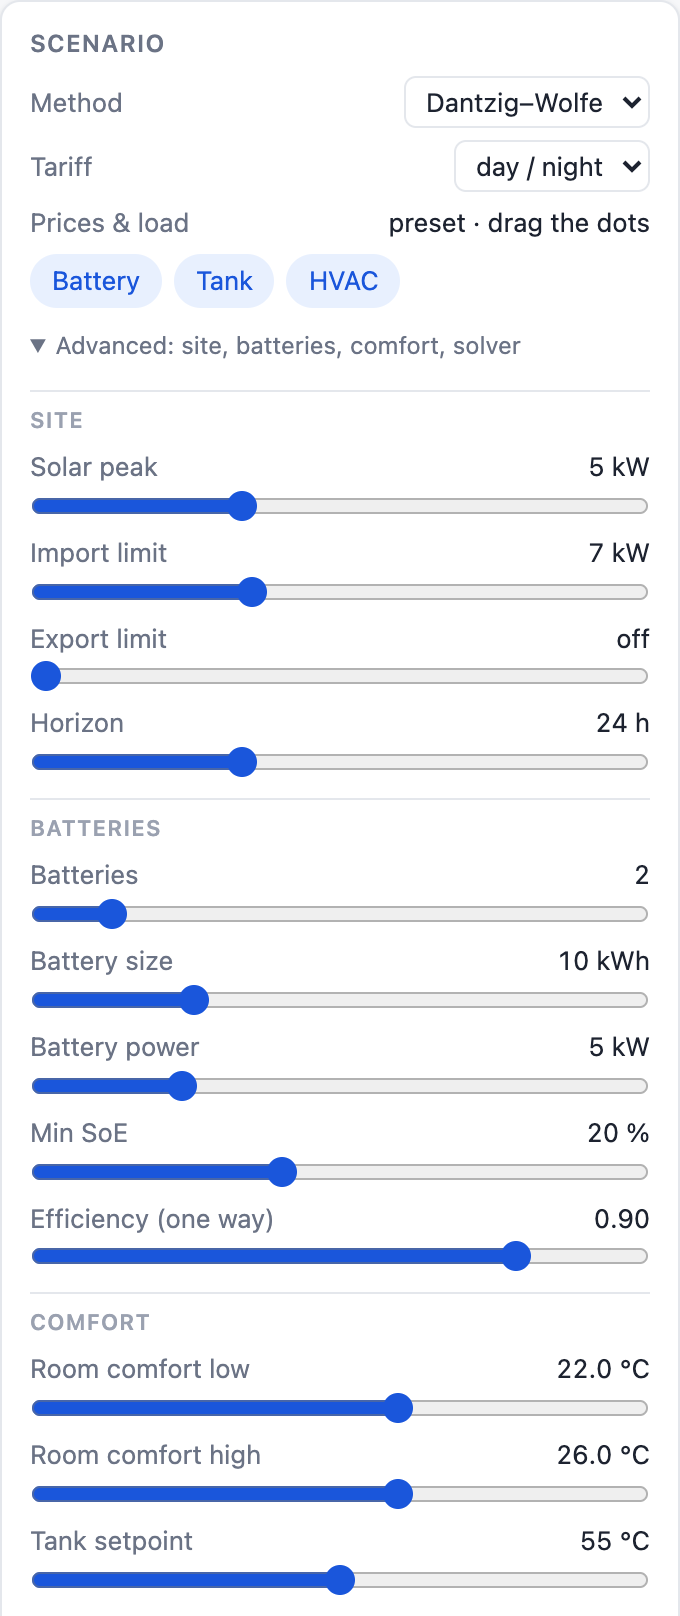
\includegraphics[width=\textwidth]{gui_dw_controls.png}
\end{minipage}\hfill
\begin{minipage}[t]{0.71\textwidth}\vspace{0pt}
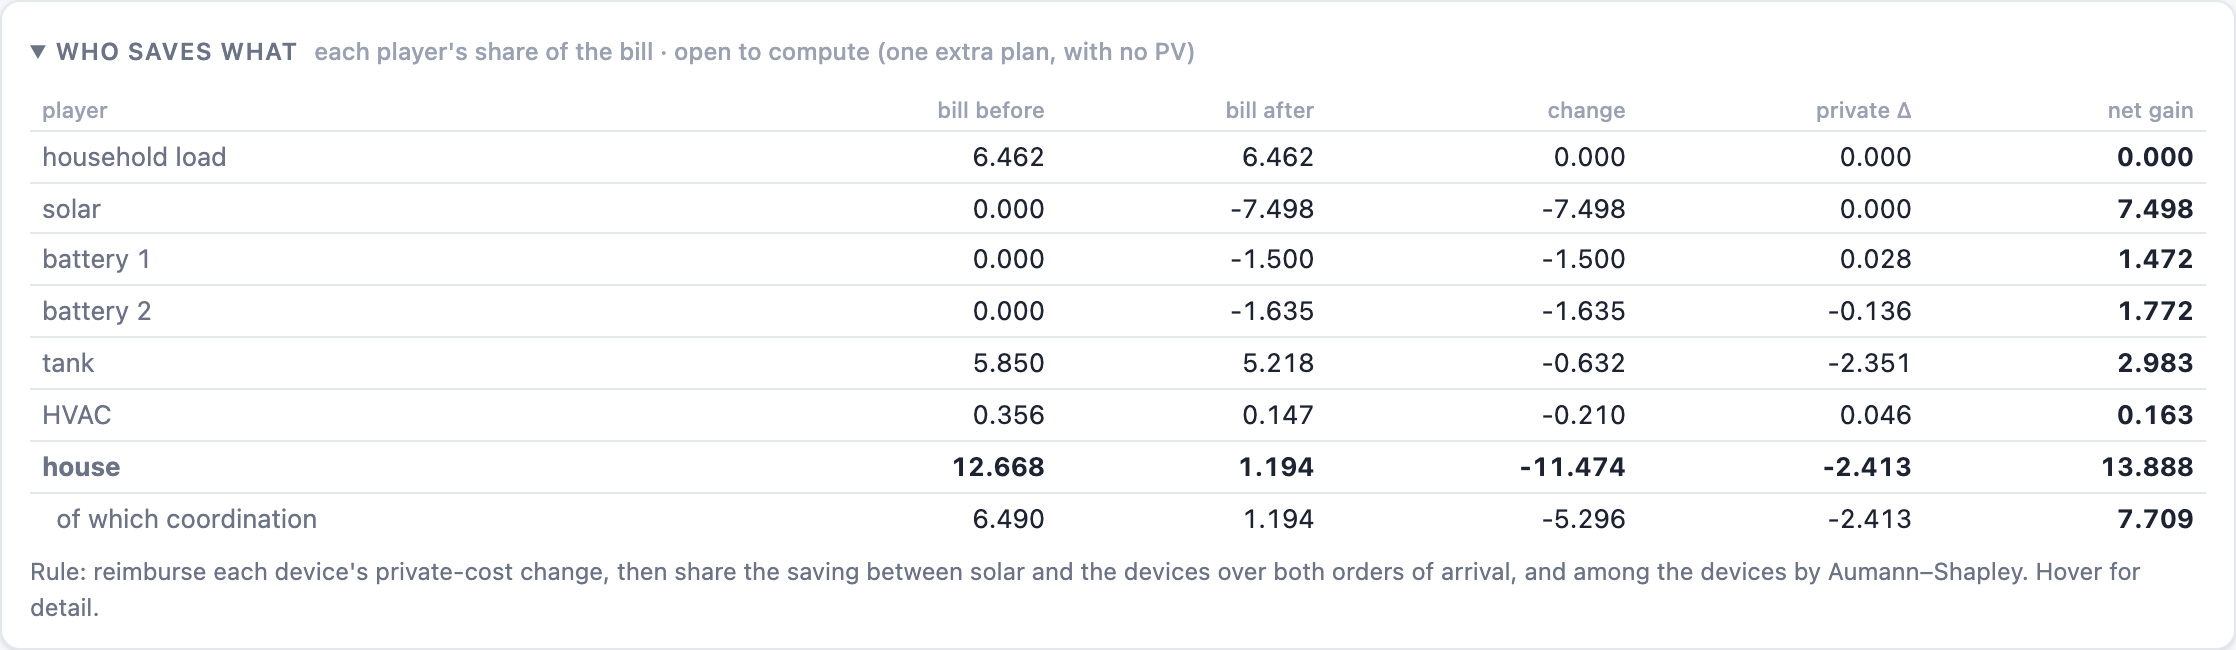
\includegraphics[width=\textwidth]{gui_dw_ledger.png}\\[4pt]
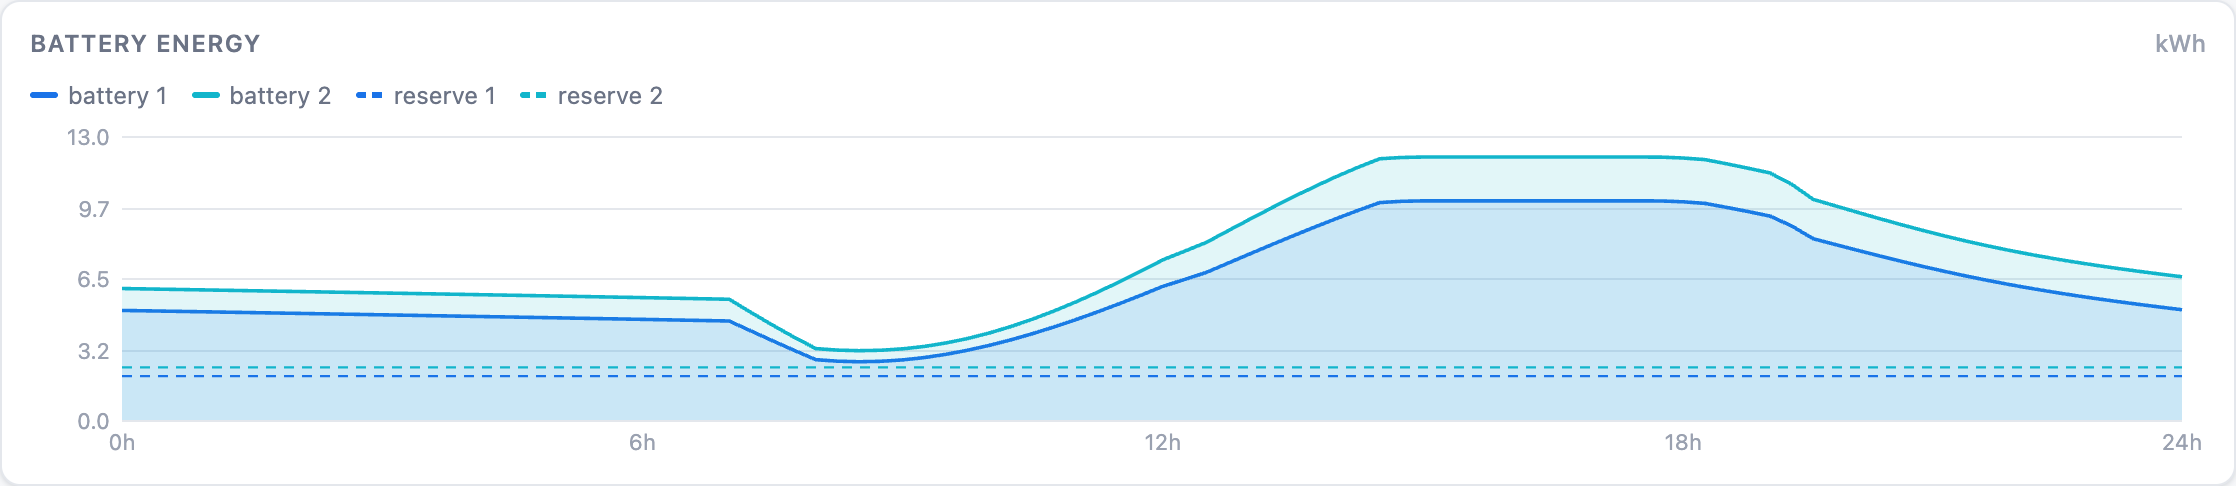
\includegraphics[width=\textwidth]{gui_dw_soc.png}
\end{minipage}
\caption{The Dantzig--Wolfe testbed: day/night tariff, two batteries with a
$20\%$ reserve, planned by Dantzig--Wolfe. Left: the controls, with
\emph{Advanced} open (the solver settings below it are not shown). Right: the
ledger, opened, and the batteries' stored energy, with the reserves dashed.
The ledger differs from Table~\ref{tab:ledger}, which uses an on/off tank; here
the tank is continuous, in the LP.}
\label{fig:guidw}
\end{figure}

\begin{figure}[htbp]
\centering
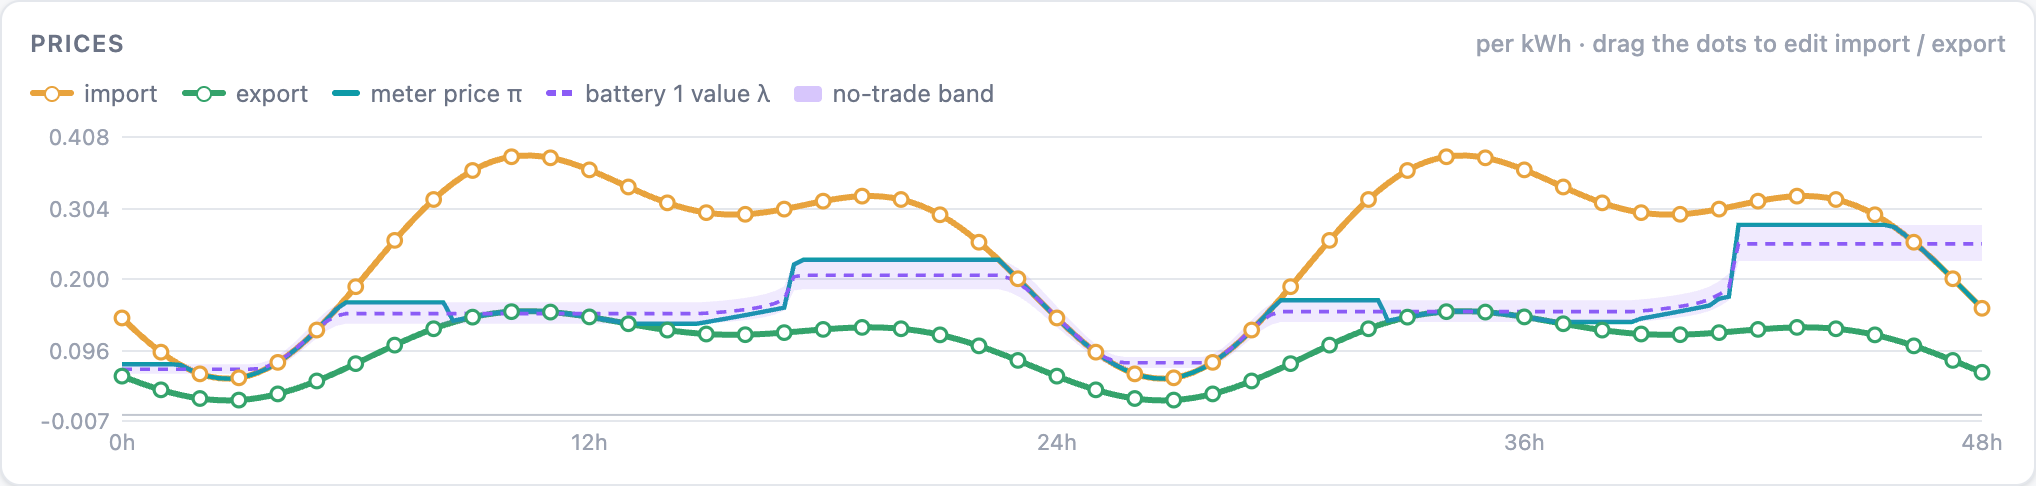
\includegraphics[width=\textwidth]{gui_reservation.png}
\caption{One battery with the tank and HVAC, a two-day dynamic tariff, planned
by Dantzig--Wolfe. $\lambda$ (dashed) sits mostly \emph{between} the export
price (green) and the import price (orange), close to the plan's meter price
$\pi$ (teal), with the shaded no-trade band of Section~\ref{sec:reservation}
around it --- import below the lower edge, export above the upper one, hold in
between; in the cheapest night hours the import price drops below the band,
and the battery charges. $\lambda$ is flat for hours at a time and steps where
the battery commits: the value function reporting that stored energy is worth
what it will fetch later, not what it costs now. At the end of the horizon it
settles at the price the plan puts on energy left in store.}
\label{fig:guireservation}
\end{figure}

\begin{figure}[htbp]
\centering
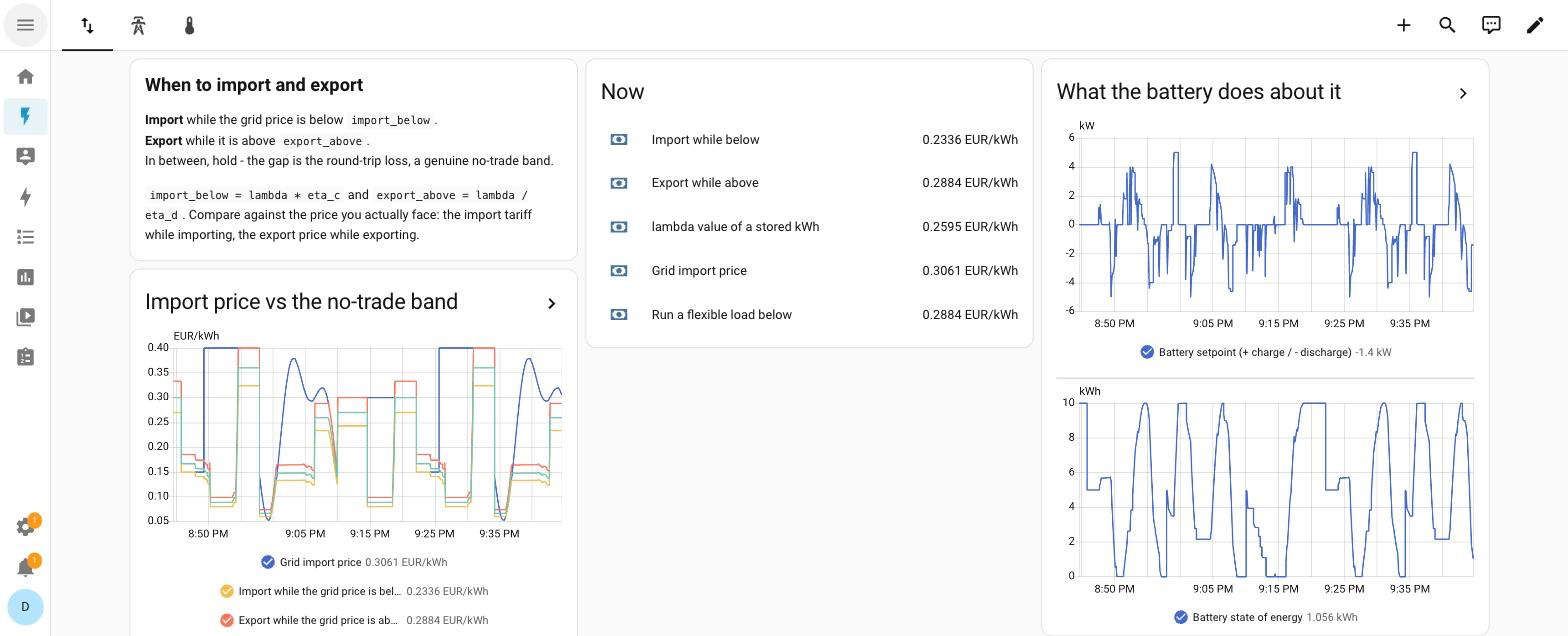
\includegraphics[width=\textwidth]{ha_dashboard.jpg}
\caption{$\lambda$ and the reservation prices streamed into Home Assistant as
plain sensor entities, sampled live. The numbers verify
\eqref{eq:bid}--\eqref{eq:ask} at a glance: $\lambda = 0.2595$, and the band runs
from $0.2336 = \lambda\Ec$ to $0.2884 = \lambda/\Ed$ at $\Ec = \Ed = 0.9$. The
prevailing import price is $0.3061$, \emph{above} the upper edge, and the battery
setpoint is correspondingly negative ($-1.4$~kW, discharging) --- the policy doing
exactly what the band says it should, with no logic in the dashboard beyond
comparing two numbers. That last point is the argument for publishing a price
rather than a schedule: any device that can read a sensor and compare it to
another can participate, without the optimiser knowing it exists.}
\label{fig:hadashboard}
\end{figure}

\section{What is guaranteed, and what is not}
\label{sec:limits}

\paragraph{Guaranteed.}
Dantzig--Wolfe's gap bounds how far any plan is from the best, up to the DP
grids (Section~\ref{sec:dw}). The joint recursion \eqref{eq:bellman} is exact
for the discretised problem.
Every state bound holds by construction, with no projection anywhere in a
transition: \eqref{eq:actionset} keeps the store inside $[\underline S,\bar S]$,
\eqref{eq:outflow} makes $\min_t T^{\infty}_t$ an exact floor for the tank, and
\eqref{eq:duty} keeps it below $\overline T$; measured over draws from $1\times$
to $200\times$ the fixture, the tank lands in $[15.000, 75.000]$ with nothing
clamped. Curtailment applied after the device solves is exact under the
conditions of Proposition~\ref{prop:curtail}. The
band \eqref{eq:band} holds at any optimum. The reservation prices
\eqref{eq:bid}--\eqref{eq:ask} follow from the definition of $\lambda$ and the
efficiency convention \eqref{eq:soe}.

\paragraph{Not guaranteed.}
\begin{itemize}[leftmargin=*]
\item \textbf{ADMM has no optimality certificate of its own.} Dantzig--Wolfe's
      bound certifies ADMM's plans too (Table~\ref{tab:compare}). ADMM converges
      for convex costs with exact steps; here the device steps are dynamic
      programmes on grids, and two of the devices are on/off
      (Table~\ref{tab:admmdiff}). Measured against a mixed-integer programme
      over the same model on the shipped grid, it forgoes $0.3$--$1.9\%$ of the
      available savings (battery and tank; Appendix~\ref{app:gaps}); on the Home
      Assistant site, $2$--$3\%$ (Table~\ref{tab:compare}).
\item \textbf{$\lambda$ is conditional.} Device $k$'s value function is solved
      against fixed $\delta^k$, so $\lambda^k$ is a marginal value given the
      other devices' plans, not a system-wide dual. Two storage units sharing a
      meter therefore need not report the same $\lambda$.
\item \textbf{Discretisation.} $\lambda$ is a numerical derivative on a finite
      grid; error against an exact dual is $0.007$--$0.032$ currency/kWh,
      shrinking as the grid refines. A $\pm 0.04$ band is published with the
      signal, and decisions inside it should not be automated.
\item \textbf{A plan may carry a small priced breach.} Dantzig--Wolfe meets a
      limit exactly or reports the breach; ADMM may leave a few watts over it
      where a device's action grid has no step that lands exactly on the
      headroom left (at most $5$~W on the test sites).
\item \textbf{The policy responds to the storage state, not to the meter.}
      Algorithm~\ref{alg:exec} takes two runtime arguments: the clock and the
      \emph{measured} storage state. Prices and the residual load $\delta$ are
      fixed at plan time and enter the value function as constants. A deviation that changes the storage state --- load running
      above forecast, draining the battery faster --- is therefore tracked,
      because the lookup lands at a different state. A deviation that does
      \emph{not} change the storage state, such as a large load switching on
      while the battery is idle, has no effect on the action until the next
      planning cycle. In particular the constraint $z_t \le \bar
      z^{\mathrm{imp}}$ is respected only in expectation over the forecast: the
      plan (through the LP under Dantzig--Wolfe, the grid connection's cost
      under ADMM) knows that
      the limit was expected to bind at a given hour, not that it is binding now. This is an approximate model-predictive scheme with feedback
      on one state variable, not a real-time constraint-enforcing controller.
      By default the package does not clip setpoints to the limit: an
      exceedance stays in place, reported and charged. Clipping against the measured meter is available as an option
      (\texttt{policy.clamp}); if used with several storage units it must
      allocate the headroom \emph{sequentially} (\texttt{clamp\_fleet}), since
      independent per-device clipping against a common measurement reproduces
      the double-counting of Section~\ref{sec:bestresponse}.
\item \textbf{The tank is one node.} \eqref{eq:tankode} assumes perfect mixing,
      and a real tank stratifies: hot water sits at the top and is drawn from
      there, so a partly reheated tank delivers water at setpoint for some time
      after its bulk mean has fallen below it. The single-node model therefore
      understates deliverable comfort during a reheat, and understates it most
      in exactly the regime the optimiser likes to sit in --- reheating late
      into a cheap window. The extension is standard (partition the tank into
      $N$ layers coupled by advection and conduction; $N = 1$ recovers
      \eqref{eq:tankode}); its cost is an $N$-dimensional state per tank.
\item \textbf{$T^{\mathrm{surr}}$ and $T^{\mathrm{in}}$ are constants.} Both are
      seasonal, and the mains is diurnal as well. Nothing in
      \eqref{eq:tankode}--\eqref{eq:duty} requires them to be constant; they are
      configuration rather than forecast only because no feed supplies them.
\item \textbf{The transition is first-order.} \eqref{eq:tank} is an explicit
      Euler step, so the within-slot path is a straight line where the truth is
      an exponential. The error vanishes at the equilibrium $T^{\infty}_t$ and
      at $\alpha_t = 0$ with no draw, and \eqref{eq:outflow} bounds it so the
      state cannot overshoot; it is largest mid-relaxation under a heavy draw.
\item \textbf{The element's binary action set is a modelling choice}, not a
      physical constraint. Over a fifteen-minute slot a thermostatic element
      cycles many times, so a duty fraction free in $[0,1]$ is at least as
      defensible; \eqref{eq:duty} already carries the machinery for it.
\end{itemize}

\section{Summary}

The problem is a finite-horizon Markov decision process whose devices are
independent except through a piecewise-linear meter cost. Solving it jointly is
exact but scales as the product of the state spaces. Solving it per device
scales linearly, and needs a coordinator.

The default coordinator, Dantzig--Wolfe, asks each device only for its best
plan at a price, mixes the plans in a small linear programme that holds the
meter, the grid limits and the linear devices exactly, and reports a lower
bound with every plan. On the Home Assistant demo site it captures $98$--$99\%$
of the available savings, at about a second per plan; it plans for both the
Home Assistant and the evcc integrations. The second, ADMM, runs as proximal
message passing --- every device responding only to one shared price, the
device DPs as its steps. It needs no LP and forgoes $2$--$3\%$ of the available
savings on the demo site, but takes an order of magnitude longer and cannot
say how far it is from the best; it is the fallback. With each battery's step
its exact LP, it reaches the optimum of a site of batteries alone.

The reason to prefer dynamic programming here is not speed of solution but the
object it produces. The value function yields a policy defined at every state,
a marginal price of stored energy, and cheap counterfactuals. From that price
follow the reservation band \eqref{eq:bid}--\eqref{eq:ask}, which says when to
trade with the grid, and the marginal cost of consumption
\eqref{eq:meterprice}, which lets a device the optimiser has never modelled
decide for itself whether to run. Coupling constraints enter as further prices
by the same mechanism, leaving the device solvers untouched.

Either plan's saving over a baseline with no PV is split among the solar and
the devices: each device is reimbursed its private-cost change, and the rest is
shared over both orders in which the solar and the devices could arrive, with
Aumann--Shapley prices among the devices. The shares add up exactly and track
the Shapley value closely, for one extra plan (Section~\ref{sec:ledger}).

\begin{thebibliography}{99}

\bibitem{owen1977}
G.~Owen.
\newblock Values of Games with a Priori Unions.
\newblock In R.~Henn and O.~Moeschlin (eds.), \emph{Mathematical Economics and
Game Theory}, Lecture Notes in Economics and Mathematical Systems 141,
pp.~76--88. Springer, 1977.
\newblock The Owen value: the Shapley value when players come in groups
(Section~\ref{sec:ledger}).

\bibitem{shapley1953}
L.~S.~Shapley.
\newblock A Value for $n$-Person Games.
\newblock In H.~W.~Kuhn and A.~W.~Tucker (eds.), \emph{Contributions to the
Theory of Games II}, Annals of Mathematics Studies 28, pp.~307--317. Princeton
University Press, 1953.
\newblock The Shapley value (Section~\ref{sec:ledger}).

\bibitem{aumannshapley1974}
R.~J.~Aumann and L.~S.~Shapley.
\newblock \emph{Values of Non-Atomic Games}.
\newblock Princeton University Press, 1974.
\newblock The continuous counterpart, used for the ledger's devices
(Section~\ref{sec:ledger}).

\bibitem{boyd2011}
S.~Boyd, N.~Parikh, E.~Chu, B.~Peleato and J.~Eckstein.
\newblock \emph{Distributed Optimization and Statistical Learning via the
Alternating Direction Method of Multipliers}.
\newblock Foundations and Trends in Machine Learning, 3(1):1--122, 2011.
\newblock The standard reference for ADMM. \S3 gives the algorithm and the
scaled form, \S3.4.1 why a varying $\rho$ should eventually be held, \S7.3.2
the exchange problem, of which \eqref{eq:exchange} is an instance.

\bibitem{goldstein2014}
T.~Goldstein, B.~O'Donoghue, S.~Setzer and R.~Baraniuk.
\newblock Fast Alternating Direction Optimization Methods.
\newblock \emph{SIAM Journal on Imaging Sciences}, 7(3), 2014.
\newblock Accelerated ADMM with a restart rule, measured here (Appendix~\ref{app:admmstable}).

\bibitem{kraning2014}
M.~Kraning, E.~Chu, J.~Lavaei and S.~Boyd.
\newblock Dynamic Network Energy Management via Proximal Message Passing.
\newblock \emph{Foundations and Trends in Optimization}, 1(2):70--122, 2013.
\newblock Proximal message passing: ADMM in exchange form for networks of energy
devices; convex relaxations for non-convex devices (Appendix~\ref{app:pmp}).

\bibitem{rivera2013}
J.~Rivera, P.~Wolfrum, S.~Hirche, C.~Goebel and H.-A.~Jacobsen.
\newblock Alternating Direction Method of Multipliers for Decentralized
Electric Vehicle Charging Control.
\newblock \emph{IEEE Conference on Decision and Control}, 2013.
\newblock ADMM for coordinating the charging of a fleet of electric vehicles.

\bibitem{wang2019}
Y.~Wang, W.~Yin and J.~Zeng.
\newblock Global Convergence of ADMM in Nonconvex Nonsmooth Optimization.
\newblock \emph{Journal of Scientific Computing}, 78, 2019.
\newblock Conditions under which ADMM converges on nonconvex problems.

\bibitem{diamond2018}
S.~Diamond, R.~Takapoui and S.~Boyd.
\newblock A General System for Heuristic Minimization of Convex Functions over
Non-Convex Sets.
\newblock \emph{Optimization Methods and Software}, 33(1), 2018.
\newblock ADMM as a heuristic over nonconvex sets.

\bibitem{dantzigwolfe1960}
G.~B.~Dantzig and P.~Wolfe.
\newblock \emph{Decomposition Principle for Linear Programs}.
\newblock Operations Research, 8(1):101--111, 1960.
\newblock The coordinator--offers scheme of Section~\ref{sec:dw}: a master over
convex combinations of the parts' proposals, priced by its simplex multipliers,
and the ``generalized programming problem'' whose columns come from arbitrary
convex sets.

\bibitem{parikh2014}
N.~Parikh and S.~Boyd.
\newblock \emph{Proximal Algorithms}.
\newblock Foundations and Trends in Optimization, 1(3):127--239, 2014.
\newblock On the proximal operator \eqref{eq:proxop} in its own right.

\bibitem{bertsekas2017}
D.~P.~Bertsekas.
\newblock \emph{Dynamic Programming and Optimal Control}, Vol.~I, 4th ed.
\newblock Athena Scientific, 2017.
\newblock The finite-horizon recursion \eqref{eq:bellman} and the interpretation
of $\partial V/\partial s$ as a costate.

\bibitem{bertsekas1989}
D.~P.~Bertsekas and J.~N.~Tsitsiklis.
\newblock \emph{Parallel and Distributed Computation: Numerical Methods}.
\newblock Prentice Hall, 1989.
\newblock Jacobi versus Gauss--Seidel block iterations and their convergence
behaviour --- the material behind Section~\ref{sec:bestresponse}.

\bibitem{chen2016}
C.~Chen, B.~He, Y.~Ye and X.~Yuan.
\newblock \emph{The direct extension of ADMM for multi-block convex minimization
problems is not necessarily convergent}.
\newblock Mathematical Programming, 155(1--2):57--79, 2016.
\newblock A divergent counterexample for three-block ADMM; the reason the device
updates of Section~\ref{sec:splitting} are not sequenced
(Remark~\ref{rem:jacobi}).

\bibitem{oneill2005}
R.~P.~O'Neill, P.~M.~Sotkiewicz, B.~F.~Hobbs, M.~H.~Rothkopf and
W.~R.~Stewart~Jr.
\newblock \emph{Efficient market-clearing prices in markets with
nonconvexities}.
\newblock European Journal of Operational Research, 164(1):269--285, 2005.
\newblock Duals of the linear programme obtained by fixing the integer variables
at their optimal values carry the usual interpretation as prices and clear the
market. The direct answer to ``a MILP has no duals''.

\bibitem{gribik2007}
P.~R.~Gribik, W.~W.~Hogan and S.~L.~Pope.
\newblock \emph{Market-Clearing Electricity Prices and Energy Uplift}.
\newblock Working paper, Harvard University, 2007.
\newblock Convex hull (minimum-uplift) pricing: prices from the Lagrangian dual
of the nonconvex problem, chosen to minimise the side-payments needed to make the
dispatch acceptable to every participant.

\bibitem{mohsenianrad2010}
A.-H.~Mohsenian-Rad and A.~Leon-Garcia.
\newblock \emph{Optimal Residential Load Control With Price Prediction in
Real-Time Electricity Pricing Environments}.
\newblock IEEE Transactions on Smart Grid, 1(2):120--133, 2010.
\newblock The reference formulation of the single-home scheduling problem: bill
plus a waiting-time discomfort term over a forecast horizon.

\bibitem{mohsenianrad2010dsm}
A.-H.~Mohsenian-Rad, V.~W.~S.~Wong, J.~Jatskevich, R.~Schober and
A.~Leon-Garcia.
\newblock \emph{Autonomous Demand-Side Management Based on Game-Theoretic Energy
Consumption Scheduling for the Future Smart Grid}.
\newblock IEEE Transactions on Smart Grid, 1(3):320--331, 2010.
\newblock The multi-household version, coordinated by a shared price.

\bibitem{hemsreview2022}
I.~Gomes, K.~Bot, M.~G.~Ruano and A.~Ruano.
\newblock \emph{Recent Techniques Used in Home Energy Management Systems: A
Review}.
\newblock Energies, 15(8):2866, 2022.
\newblock Survey of the MILP-dominated HEMS literature and its variants.

\bibitem{pereira1991}
M.~V.~F.~Pereira and L.~M.~V.~G.~Pinto.
\newblock \emph{Multi-stage stochastic optimization applied to energy planning}.
\newblock Mathematical Programming, 52(1--3):359--375, 1991.
\newblock Stochastic dual dynamic programming. The future-cost function whose
slope is the value of stored water is the direct ancestor of $\lambda$.

\bibitem{philpott2017}
A.~B.~Philpott.
\newblock \emph{On the Marginal Value of Water for Hydroelectricity}.
\newblock In \emph{Advances and Trends in Optimization with Engineering
Applications}, SIAM, 2017.
\newblock What a water value is, what it is conditional on, and how it is misread
in practice.

\bibitem{vandeven2012}
P.~M.~van~de~Ven, N.~Hegde, L.~Massouli\'e and T.~Salonidis.
\newblock \emph{Optimal control of end-user energy storage}.
\newblock arXiv:1203.1891, 2012.
\newblock Proves that the optimal end-user storage policy has a threshold
structure, with thresholds moving with price --- the formal statement of the
reservation band \eqref{eq:bid}--\eqref{eq:ask}.

\end{thebibliography}

\appendix

\section{What the suboptimality looks like}
\label{app:gaps}

The percentages quoted throughout are small fractions of a quantity that is
itself modest, which makes them easy to misread in either direction. These plots
show the trajectories behind the numbers. All are produced by
\texttt{bench/make\_theory\_figs.py} on the shipped $24$~h fixtures at
$\dt = 0.25$~h; ``capture'' is the fraction of available savings (baseline minus
exact) that the fast path realises, so $100\%$ is the exact optimum and the
distance below it is what was forgone. The coordinator in these figures is
ADMM, which has no bound of its own; Dantzig--Wolfe's plans carry their
certificate (Section~\ref{sec:dw}).

\begin{figure}[htbp]
\centering
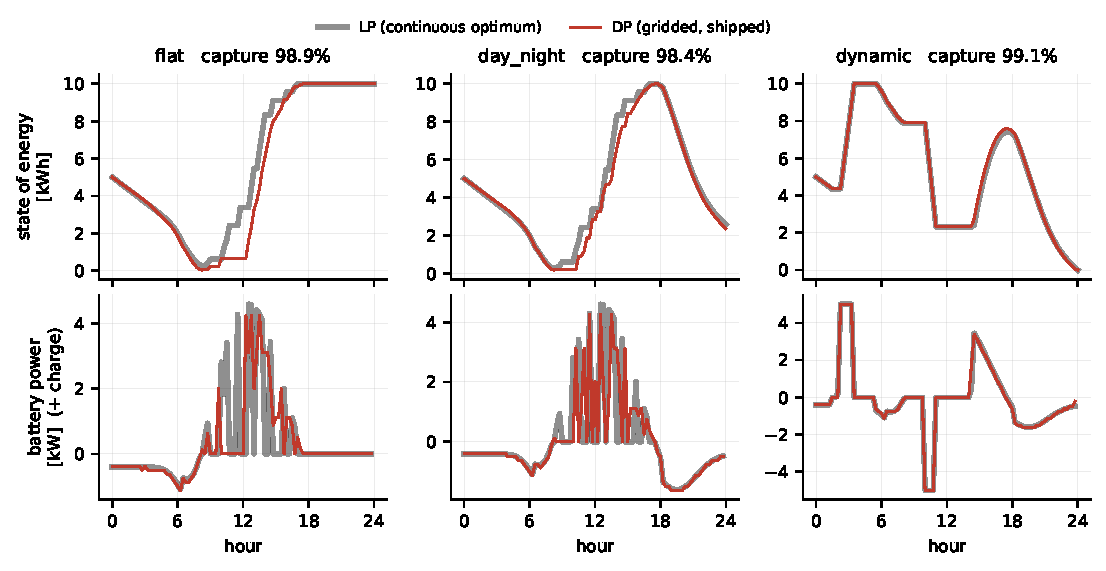
\includegraphics[width=\textwidth]{gap_discretisation.pdf}
\caption{\textbf{Discretisation.} The shipped battery DP (red) against the exact
continuous LP (grey), on the same model. The staircase in the state-of-energy row
is the finite state grid, and it is the whole of the error --- the two solutions
agree on \emph{what} to do and disagree only on the last increment of \emph{how
much}. On the dynamic tariff the traces are visually indistinguishable. Capture
$98.4$--$99.2\%$; the residual is tunable by refining the grid, at a cost in
solve time.}
\label{fig:gapdisc}
\end{figure}

\begin{figure}[htbp]
\centering
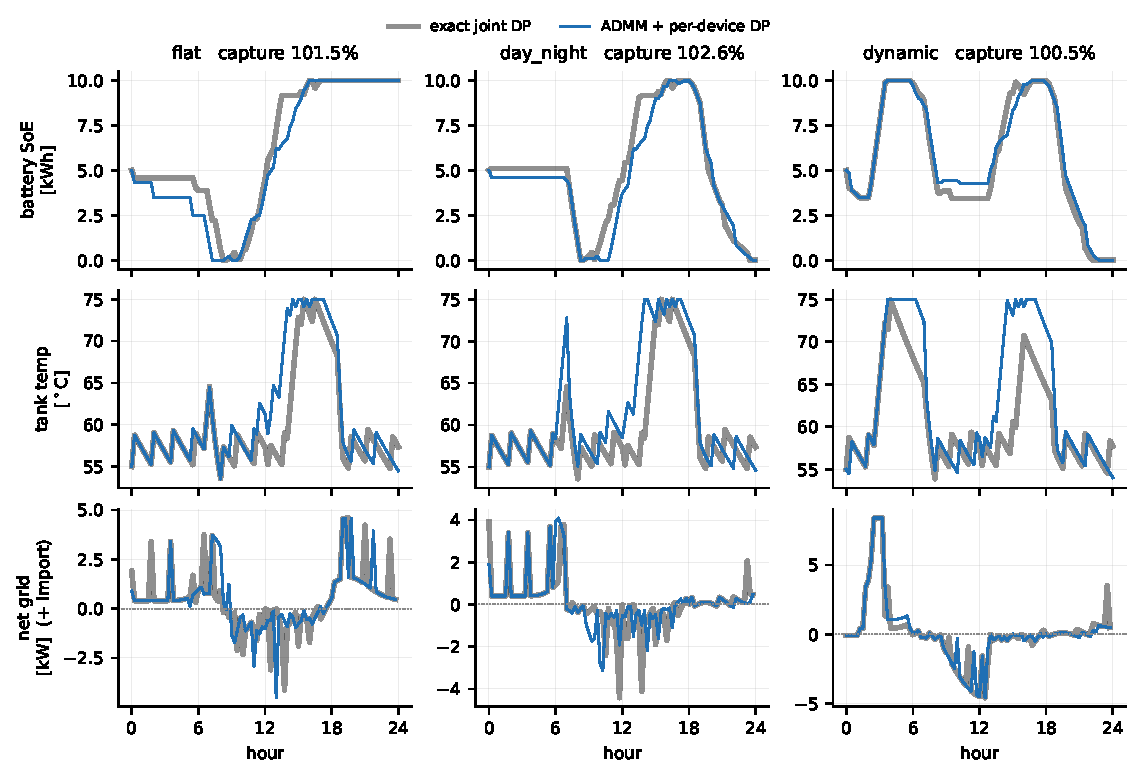
\includegraphics[width=\textwidth]{gap_decomposition.pdf}
\caption{\textbf{Decomposition.} ADMM with per-device DPs (blue) against the
joint recursion over the product state space (grey), for a battery and a water
heater, on the same $50$-state battery grid. The strategies are the same shape
--- discharge overnight, refill on PV, heat the tank into the surplus --- and
differ mostly in timing, and in how hot the tank is taken. Capture $100.5$ to
$102.6\%$: ADMM's plans are slightly cheaper than the joint recursion's, which
is exact only for its own discretisation --- scored on the model itself, its
plan is not the optimum. That makes it the wrong yardstick at this precision;
Figure~\ref{fig:gapsum} adds the right one, a MILP over the same model.}
\label{fig:gapdec}
\end{figure}

\begin{figure}[htbp]
\centering
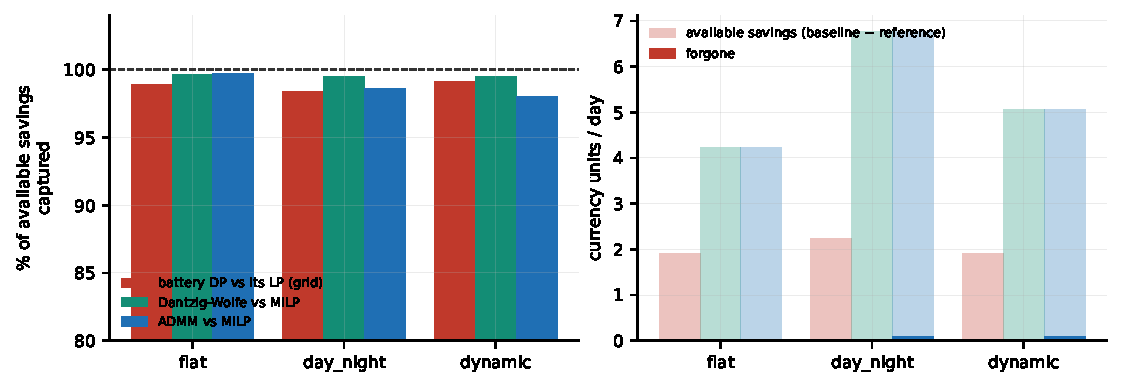
\includegraphics[width=\textwidth]{gap_summary.pdf}
\caption{\textbf{What the percentages are percentages of.} Left: capture by
tariff --- the battery DP against the continuous LP (red), ADMM against the
joint recursion (blue), and ADMM on the shipped battery grid against a MILP
over the same model, which counts both losses at once (green): $98.1$ to
$99.7\%$. Right: the same result in money --- the pale bar is the savings
available over an uncontrolled baseline, the solid bar the part the fast path
forgoes (below zero where it beats its reference). The red bars are the
battery-only site, the others the battery-plus-water-heater site, so the pale
bars are not meant to match: different sites have different amounts to win.
The point of the panel is the ratio within each bar. Read together with Figure~\ref{fig:gapdec}, the claim being made is
narrow: this loses a visible slice of the \emph{improvement}, while capturing the
large majority of it and producing, as a by-product, a price defined at every
state rather than only along the planned trajectory
(Section~\ref{sec:milpduals}).}
\label{fig:gapsum}
\end{figure}

\section{Scaling with device count}
\label{app:scale}

Section~\ref{sec:decomposition} claims the decomposition trades optimality for
a cost that is linear in the device count, against a joint recursion that is
exponential in it. Figure~\ref{fig:scaling} measures the first half of that
claim directly, from one storage unit to twenty, each with $100$ state and $41$
action grid points, over $96$ slots, alongside the two thermal devices.

\begin{figure}[htbp]
\centering
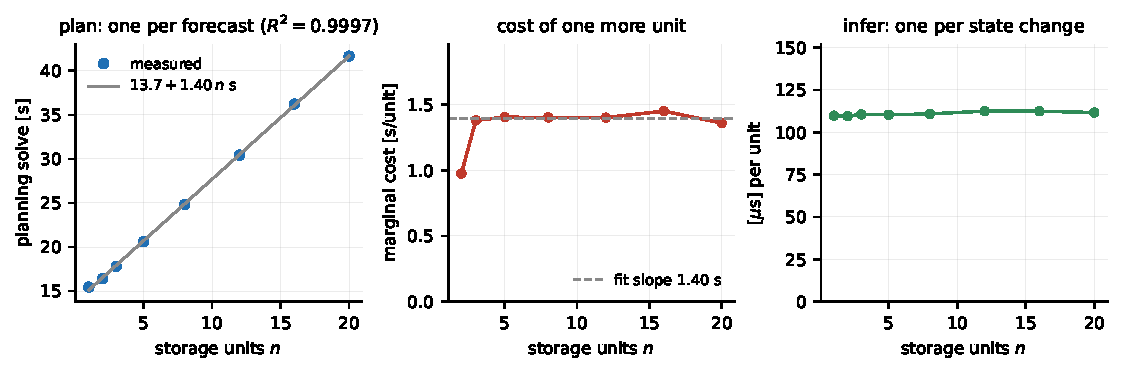
\includegraphics[width=\textwidth]{scaling.pdf}
\caption{Solve cost against the number of storage units $n$, planned by ADMM
($100$ iterations). \textbf{Left:} the planning solve is affine in $n$
($R^2 = 0.9997$), $13.7 + 1.40\,n$ seconds; the intercept is the two thermal
devices --- relaxed while iterating, and re-planned as themselves every
iteration --- and the fixed overhead, which is why the fit is stated in storage
units rather than in total devices. \textbf{Centre:} the same claim in the form
that cannot flatter itself --- the cost of adding one more unit, flat at
$\approx 1.4$~s from the third unit on rather than growing. \textbf{Right:} the
execution tier, $110$--$113\,\mu$s per unit, nearly independent of fleet size,
timed at four full coordination sweeps with early exit disabled so the figure
is a worst case rather than a convergence artefact.}
\label{fig:scaling}
\end{figure}

Twenty storage units plan in $42$~s and decide in $2.2$~ms (one machine; times
vary between runs). Dantzig--Wolfe plans the same sites in $0.6$ to $4.3$~s,
from one unit to twenty: its iterations are few, and its master LP, which holds
the batteries, grows with them. Against a
planning cadence of $5$--$15$ minutes and an execution tier that must answer
within a control period, neither is a constraint; the binding limit on device
count is elsewhere, in the growth of the decomposition gap that
Appendix~\ref{app:gaps} measures at two devices and does not extrapolate.

The contrast with the exact joint recursion is not a matter of constant
factors. Its state space is the product of the individual ones, so at $100$
points per unit it is $10^4$ states at two units, $10^6$ at three, and $10^{40}$
at twenty. The decomposition is not faster than the joint solve at twenty
units; the joint solve does not exist at twenty units.

\section{The Dantzig--Wolfe master, pricing problem and bound}
\label{app:dw}

This appendix states Section~\ref{sec:dw} precisely, as
\texttt{dw/coordinator.py} implements it.

\paragraph{Sets.}
Bidding devices $k \in \mathcal K$, each with a pool $\mathcal J_k$ of offers;
offer $j$ has power profile $p^{kj} \in \R^n$ and private cost $f_{kj}$
(comfort, horizon-edge energy, SoC-goal shortfall). LP storage units
$b \in \mathcal B$, with charge $c^b_t$, discharge $e^b_t$ and state $s^b_t$.

\paragraph{Master.}
With $z^{\pm}_t$ import and export within the limits, $o^{\pm}_t \ge 0$ their
breaches, $\chi_t \in [0, g_t]$ curtailment, and $\lambda_{kj} \ge 0$ the
weights,
\begin{equation}
\begin{aligned}
\min\;& \dt\sum_t \Big(c^{\mathrm{imp}}_t z^+_t + (c^{\mathrm{imp}}_t + c^{\mathrm{br}})\, o^+_t
   - c^{\mathrm{exp}}_t z^-_t - (c^{\mathrm{exp}}_t - c^{\mathrm{br}})\, o^-_t\Big) \\
 & \quad + \textstyle\sum_{k,j} f_{kj}\lambda_{kj} - \sum_b \pi_{\mathrm T}\, s^b_n \\
\text{s.t.}\;& z^+_t + o^+_t - z^-_t - o^-_t - \chi_t
   - \textstyle\sum_{k,j} p^{kj}_t\lambda_{kj} - \sum_b (c^b_t - e^b_t) = d_t
   && [\pi_t\dt] \\
& \textstyle\sum_{j \in \mathcal J_k} \lambda_{kj} = 1 && [\sigma_k] \\
& s^b_{t+1} = s^b_t + \dt\,(\Ec c^b_t - e^b_t/\Ed), \\
& 0 \le c^b_t \le \bar P_{\mathrm c},\quad 0 \le e^b_t \le \bar P_{\mathrm d},\quad
  \underline S \le s^b_t \le \bar S ,
\end{aligned}
\label{eq:dwmaster}
\end{equation}
with $0 \le z^+ \le \bar z^{\mathrm{imp}}$, $0 \le z^- \le \bar z^{\mathrm{exp}}$.
The bracketed symbols are the duals. The meter row's dual, divided by $\dt$, is
the meter price $\pi_t$ in currency per kWh. Two properties make this master
easy to use. The kink of \eqref{eq:bill} is exact without a binary, because
$z^+$ and $z^-$ carry different prices and, when $c^{\mathrm{exp}} \le
c^{\mathrm{imp}}$, an optimum never uses both. And the master is always
feasible, since the breach variables absorb any imbalance, so any single offer
per device starts it. A modulating tank enters as LP variables too, with the
dynamics \eqref{eq:tank} at a continuous duty; it is omitted above for brevity.

\paragraph{Pricing.}
At duals $(\pi, \sigma)$, device $k$'s best offer solves
\begin{equation}
  \min_{p^k \in \mathcal P^k}\; f_k(p^k) + \dt\,\pi^{\!\top} p^k \;-\; \sigma_k ,
  \label{eq:dwpricing}
\end{equation}
which is the device's own dynamic programme with import and export prices both
set to $\pi$ and no residual load. A negative value is a new offer. The
comfort reference price and the battery terminal price are held at their tariff
values, not recomputed from $\pi$, so that the DP optimises the same $f_k$ the
master charges.

\paragraph{Bound.}
For any $\pi$,
\begin{equation}
  \begin{aligned}
  L(\pi) \;=\;& \dt\,\pi^{\!\top} d
  \;+\; \sum_{k} \min_{p^k}\big(f_k(p^k) + \dt\,\pi^{\!\top}p^k\big)
  \;+\; \sum_b \min_{\text{unit } b}\big(\dt\,\pi^{\!\top}(c^b - e^b) - \pi_{\mathrm T} s^b_n\big) \\
  &+\; \sum_{v}\sum_t \min_{u_{v,t}} \big(\mathrm{cost}_{v,t} - \pi_t\dt\, a_v\big)u_{v,t}
  \;\;\le\;\; J^\star ,
  \end{aligned}
  \label{eq:dwbound}
\end{equation}
where the last sum runs over the meter variables $v \in \{z^\pm, o^\pm, \chi\}$,
each with meter-row coefficient $a_v = \pm 1$ and box bounds, so its minimum is
at a bound and is closed form. This is the Lagrangian relaxation of the meter
row, and weak duality gives the inequality. Outside
$[\min(c^{\mathrm{exp}}_t, 0),\, c^{\mathrm{imp}}_t]$, widened by
$c^{\mathrm{br}}$ where a limit binds, $L$ falls steeply, so the useful prices
are naturally bounded. The code evaluates $L$ at every price it has used, takes each
device's minimum over the DP's answer \emph{and} every offer seen at that price
--- the DP is exact only on its grid --- and reports the best.

\paragraph{Recovery.}
Re-solve \eqref{eq:dwmaster} with $\lambda_{kj} \in \{0,1\}$ for every device
that cannot run a blend, keeping the LP units and a modulating tank continuous.
This is price-and-branch: a branch and bound over ``one offer per device'',
branching on the most fractional device (\texttt{dw/lpsolver.py}). The plan's
cost $J(\text{plan})$ is then evaluated on the full objective, and
$J(\text{plan}) - \max_\pi L(\pi)$ is the reported gap.

\paragraph{Batteries that bid.}
A battery goes into the master only if it is plain: no per-slot charge floor,
no SoC goal, no charger minimum, no SoC gate. Otherwise it is a bidding device.
Its private cost adds the DP's penalties to the terminal term,
$f(s) = \pi_{\mathrm T}(s_0 - s_n) + \kappa_{\mathrm{goal}}\sum_t [s^{\mathrm{goal}}_t - s_t]^+
+ (\text{gate penalties})$, exactly as \texttt{solve\_battery} subtracts them from
$V_t$, so the master and the pricing DP optimise the same function.

\section{ADMM on the test sites}
\label{app:admmstable}

\texttt{bench/admm\_stability.py} runs Algorithm~\ref{alg:plan} on $72$ sites
--- the three tariffs, one to three batteries, a $7$~kW import limit or none,
$5$ or $8$~kW of PV, $10$ or $20$~kWh per battery, a $50$-state battery grid,
$48$~hours --- and scores every plan against the Dantzig--Wolfe lower bound,
by \texttt{DWCoordinator.parts}, the basis the bound is stated on. Twelve of
the sites (each tariff, one or three batteries, a limit or none; $5$~kW of PV,
$10$~kWh per battery) are where the variants were compared
(\texttt{bench/exchange\_tune.py}).

\begin{table}[htbp]
\centering
\small
\begin{tabular}{lrrrrr}
\toprule
& \multicolumn{2}{c}{mean above bound} & & & \\
\cmidrule(lr){2-3}
& limit & no limit & worst & converged & time \\
\midrule
ADMM, $72$ sites & $0.538$ & $0.478$ & $1.056$ & $16$ of $72$ & $46$~s \\
\bottomrule
\end{tabular}
\caption{Algorithm~\ref{alg:plan} on the $72$ sites ($36$ with a limit), distance
above the Dantzig--Wolfe lower bound in currency per day. Time is per site, six
sites at a time on one machine. Dantzig--Wolfe on the same sites:
$0.10$ (Table~\ref{tab:pmp}).}
\label{tab:admm72}
\end{table}

\noindent
Seven of the $72$ plans exceed the import limit, by at most $5$~W, and pay the
breach price for it.

\paragraph{What each departure is worth.} On the twelve sites, one change at a
time against the method as shipped (the rows of Table~\ref{tab:admmdiff} in
brackets):

\begin{center}
\small
\begin{tabular}{lrrrr}
\toprule
& above bound & worst & converged & time \\
\midrule
as shipped                                  & $0.416$ & $0.813$ & $6$ of $12$ & $42$~s \\
tank and HVAC not relaxed (2)               & $1.280$ & $1.930$ & $6$ & $9$~s \\
relaxed to quarters, not twelfths (2)       & $0.438$ & $0.861$ & $4$ & $22$~s \\
no polish (5)                               & $1.987$ & $3.983$ & $6$ & $41$~s \\
no baseline fallback (5)                    & $0.416$ & $0.813$ & $6$ & $41$~s \\
kink not rounded (6)                        & $0.397$ & $0.817$ & $2$ & $44$~s \\
$300$ iterations, not $100$ (8)             & $0.392$ & $0.719$ & $6$ & $87$~s \\
momentum with restart                       & $0.416$ & $0.813$ & $6$ & $45$~s \\
LP battery steps (1)                        & $0.439$ & $0.726$ & $8$ & $29$~s \\
\bottomrule
\end{tabular}
\end{center}

\noindent
The relaxation and the polish carry the method. Without the relaxation the
on/off devices can only jump by a whole element (Remark~\ref{rem:binary}), and
the plans end three times as far from the bound; quarters instead of twelfths
halve the time for a slightly worse plan. Without the polish, the best runnable
plan the iterations produce sits $2.0$ above the bound: the iterations find a
plan from which one device at a time can improve a long way, not a plan that is
good by itself. The baseline fallback changes nothing here; it is a safety net.
Rounding the kink trades a little quality for convergence: three times as many
runs pass the stopping test, for plans $0.02$ further from the bound. Three
hundred iterations come $0.02$ closer than a hundred, at twice the time.
Nesterov momentum with restart \cite{goldstein2014}, which the code offers
(\texttt{exchange\_momentum}), changes nothing.

$\rho$ matters more to speed than to quality. With exact device steps
(\texttt{bench/rho\_sweep.py}), a starting $\rho$ of $0.03$--$0.1$ converged in a
median of $80$--$115$ iterations, adapted or held fixed, and a starting $\rho$
of $3$ in $250$--$770$; with a large $\rho$ the residual test was met while the
plan was still up to $0.78$ from the optimum, the tether holding plans nearly
still --- one reason the best plan seen is kept, not the last (row~4).

\paragraph{Many batteries.} On a site with eight batteries ($10$ to $28$~kWh,
dynamic tariff, $7$~kW import limit, $24$~h) the iterations do not settle: the
primal residual stalls near $2.5$, against a stopping threshold of $0.04$, and
the best plan, $1.0$ above the bound, is found by iteration $13$; $300$
iterations find nothing better. With every step solved exactly as a QP ---
continuous batteries, the tank and HVAC relaxed --- the same site converges in
$41$ iterations (\texttt{bench/many\_batteries.py}).

The difference is the one the convergence proof turns on. It needs every cost
to be convex \cite[\S3.2]{boyd2011}: its key step \cite[App.~A,
(A.2)]{boyd2011} infers from ``$x$ minimises $f$ plus the square'' that ``$x$
minimises $f$ plus a linear term'', which holds only for convex $f$; and errors
in the steps are tolerated only if they are summable \cite[\S3.4.4]{boyd2011}.
A battery on a grid is neither convex nor summably inexact: however little the
price moves, its plan moves by a whole power step or not at all, and the error
never shrinks. Kraning et al.\ say as much for non-convex devices: no guarantee
that the method converges, ``or even that it converges at all''
\cite{kraning2014}. With exact steps, a battery's plan moves continuously with
the price, so the total does too, and the price can settle where the house
balances even when every battery sits on the same margin. With grid steps, one
battery alone converges (in $85$ iterations). Several facing one price reach
their switching points together: wherever the plans still move, all eight
batteries move at once, and all the same way, so the total jumps by about
eight power steps, overshoots the balance, and the price turns them all back.
The stall grows with the number of batteries and with the power step:

\begin{center}
\small
\begin{tabular}{rrrr}
\toprule
batteries & power step & residual, last $20$ iterations & batteries moving at once \\
\midrule
$1$ & $0.40$~kW & $0.06$ (converged) & --- \\
$2$ & $0.40$~kW & $0.36$ & $1.5$ of $2$ \\
$4$ & $0.40$~kW & $0.75$ & $2.0$ of $4$ \\
$8$ & $0.40$~kW & $2.46$ & $8$ of $8$ \\
$8$ & $0.20$~kW & $1.40$ & $8$ of $8$ \\
$8$ & $0.10$~kW & $0.76$ & $8$ of $8$ \\
\bottomrule
\end{tabular}
\end{center}

\noindent
A finer grid shrinks the stall in proportion but does not remove it; exact
battery steps do. Dantzig--Wolfe, which holds the batteries as exact variables
in its LP, comes within $0.05$ of the same bound in $2.3$~s.

\paragraph{Exact battery steps.} Taking each battery's step as its LP, solved
exactly (Section~\ref{sec:exchange}), removes the lockstep: the eight-battery
site converges, in $86$ iterations ($38$ with the kink unrounded), where with
DP steps it never does. The plan is no better for it --- $0.93$ above the bound
($0.84$ unrounded) --- because the tank and HVAC are still on/off. On the $72$
sites $49$ runs converge instead of $16$, in about two-thirds of the time, but
the plans end slightly further from the bound ($0.54$ against $0.51$; worst
$1.23$ against $1.06$): converging does not make the on/off devices' plans any
better.
Where every step is exact and convex --- three batteries alone, the kink
unrounded --- the loop converges to the optimum, as the theorem says, to within
what its stopping test asks:

\begin{center}
\small
\begin{tabular}{lrr}
\toprule
stopping tolerance $\epsilon^{\mathrm{abs}}$ & iterations & above the optimum \\
\midrule
$10^{-3}$ (the default) & $110$ & $0.049$ \\
$10^{-4}$ & $248$ & $0.006$ \\
$10^{-5}$ & $847$ & $0.001$ \\
$10^{-6}$ & $3000$ (the cap) & $0.0001$ \\
\bottomrule
\end{tabular}
\end{center}

\noindent
The optimum is the Dantzig--Wolfe master's, which holds the batteries exactly
and closes its gap on this site.

\paragraph{Warm starts} (\texttt{bench/warm\_start.py}). Starting each LP
battery step from its previous solution takes a third of the time out of those
steps, with the same plans; a solve of three batteries alone falls from $0.8$
to $0.5$~s, one with the tank and HVAC by $1$--$5\%$, since most of its time
is the thermal devices'. Starting a solve from the last one's best state after
one setting changes --- PV $5 \to 6$~kW, a battery $10 \to 12$~kWh, the import
limit $7 \to 6$~kW; one or two batteries; DP or LP steps; twelve cases --- the
runnable plan came within $0.05$ of the run's best by iteration $21$ on
average, against $65$ cold; six runs converged instead of one, and the solves
took $15$~s instead of $21$~s. The final plans were as good on average ($0.222$
above the bound against $0.223$), though single cases moved by up to $0.09$
either way. One planning cycle later --- the forecast one slot on, the state
shifted with it; four cases --- the plan was near its best by iteration $15$
against $64$, in a third less time, and ended $0.02$ further from the bound on
average: a warm start can settle near the previous solution when a better one
lies elsewhere.

\paragraph{Is it the on/off devices?} Only partly. Letting the tank and HVAC
run twelfths of a slot in the problem itself (\texttt{bench/relaxed\_devices.py})
makes it nearly convex: Dantzig--Wolfe's gap falls from $0.10$ to zero within
its grids. On those relaxed sites, proximal message passing with the DPs as its
device steps (\texttt{bench/pmp\_dp.py}) still converged on only $10$ of the
$72$ within $300$ iterations, and its plans, polished, end $0.25$ above the
bound, against $0.51$ on the real sites (Table~\ref{tab:admm72}). With exact
steps it converges everywhere (Appendix~\ref{app:pmp}). So the gridded steps
keep the DP version from converging and account for roughly half its distance
from the bound; the on/off devices account for the other half, which
Dantzig--Wolfe closes by choosing among their plans together.

\section{Proximal message passing on these sites}
\label{app:pmp}

Proximal message passing \cite{kraning2014} is ADMM in exchange form for a
network of devices joined by nets. In each iteration every device, in
parallel, finds the plan that minimises its own cost plus
$(\rho/2)\|p - (p^{\mathrm{prev}} - \bar p - u)\|^2$, where $\bar p$ is its
net's average power imbalance and $u$ the net's scaled price; then every net
averages its imbalance and sets $u \leftarrow u + \bar p$. For convex devices it
converges to the optimal plans and prices. For non-convex devices the paper
runs it on convex relaxations, whose optimum is a lower bound, and leaves open
how to build runnable plans from the result.

\paragraph{Set-up.} The house is one net. Its devices are the fixed load; the
PV, curtailable at no cost; the grid connection, the paper's ``external tie'',
with import and export prices and the breach price beyond a limit; each
battery, continuous; and the tank and HVAC, relaxed to a modulating element and
to heat and cool duties $h, k \ge 0$ with $h + k \le 1$. Every prox is solved
exactly as a small QP. $\rho$ follows the paper's controller, with
$\lambda = \mu = 0.01$ (the paper gives $10^{-3}$--$10^{-1}$ as typical) and held
after $200$ iterations, and iterations stop at the paper's
residual test with $\epsilon^{\mathrm{abs}} = 10^{-3}$. Two ways to recover a
runnable plan were scored, both ours: each on/off device re-plans at the
relaxed prices while the batteries keep their relaxed plans (``prices
only''); and that, followed by the testbed's polish.

\begin{table}[htbp]
\centering
\small
\begin{tabular}{lrrrr}
\toprule
& \multicolumn{3}{c}{mean above bound} & \\
\cmidrule(lr){2-4}
method & all & limit & no limit & time \\
\midrule
Dantzig--Wolfe                       & $0.099$ & $0.103$ & $0.096$ & $4.8$~s \\
ADMM (Algorithm~\ref{alg:plan})     & $0.508$ & $0.538$ & $0.478$ & $46$~s \\
message passing, prices only         & $3.869$ & $5.326$ & $2.411$ & \\
message passing, then polish         & $0.451$ & $0.465$ & $0.438$ & $13.3$~s \\
\bottomrule
\end{tabular}
\caption{The $72$ sites of Appendix~\ref{app:admmstable}, every plan scored by
\texttt{DWCoordinator.parts}, the basis of the Dantzig--Wolfe bound
(\texttt{bench/prior\_art.py}, which needs \texttt{osqp}). Message passing
converged on all $72$, in $101$ iterations on average; its time includes both
recoveries. Times are from separate runs: Dantzig--Wolfe and message passing
one site at a time, ADMM six at a time (Table~\ref{tab:admm72}).}
\label{tab:pmp}
\end{table}

\paragraph{What it shows.} Message passing converged everywhere, in line with
the under-$200$ iterations the paper reports for its convex networks. Its
relaxed optimum lies on average $0.48$ below the Dantzig--Wolfe bound,
consistent with a fractional on/off element being a looser relaxation than
Dantzig--Wolfe's blends of runnable plans (the two also differ in how finely
they grid the thermal devices). Recovering by prices alone fails: wherever
the relaxation runs a device at a fraction, the relaxed price leaves the on/off
device nearly indifferent, so it rounds up or down on its own. On the worst
site the relaxation runs the tank at a fraction in $160$ of $192$ slots; at the
relaxed prices the on/off tank instead runs at full power in $54$, half of them
where the relaxation ran it below half power, on top of battery plans made for
the fractional tank --- and the plan overshoots the $7$~kW limit by
$2.8$~kWh.
Starting the polish from the relaxed plans comes to $0.45$ above the bound,
against $0.51$ for Algorithm~\ref{alg:plan}, whose gridded DP steps rarely
converge --- and part of that lead is the continuous batteries, where the DPs'
sit on a $50$-state grid. The lesson is the one the rest of the paper draws:
what closes the gap is solving the convex part jointly and exactly, then
choosing the discrete actions together, not through a price. Dantzig--Wolfe
does both, faster, and certifies the result. ADMM (Section~\ref{sec:exchange})
runs the same method with the DPs as device steps, and so without any solver.

\end{document}
